%%% Title:    Overview of Linear Regression
%%% Author:   Kyle M. Lang
%%% Created:  2018-04-12
%%% Modified: 2021-11-03

\documentclass[10pt]{beamer}\usepackage[]{graphicx}\usepackage[]{color}
% maxwidth is the original width if it is less than linewidth
% otherwise use linewidth (to make sure the graphics do not exceed the margin)
\makeatletter
\def\maxwidth{ %
  \ifdim\Gin@nat@width>\linewidth
    \linewidth
  \else
    \Gin@nat@width
  \fi
}
\makeatother

\definecolor{fgcolor}{rgb}{0, 0, 0}
\newcommand{\hlnum}[1]{\textcolor[rgb]{0.69,0.494,0}{#1}}%
\newcommand{\hlstr}[1]{\textcolor[rgb]{0.749,0.012,0.012}{#1}}%
\newcommand{\hlcom}[1]{\textcolor[rgb]{0.514,0.506,0.514}{\textit{#1}}}%
\newcommand{\hlopt}[1]{\textcolor[rgb]{0,0,0}{#1}}%
\newcommand{\hlstd}[1]{\textcolor[rgb]{0,0,0}{#1}}%
\newcommand{\hlkwa}[1]{\textcolor[rgb]{0,0,0}{\textbf{#1}}}%
\newcommand{\hlkwb}[1]{\textcolor[rgb]{0,0.341,0.682}{#1}}%
\newcommand{\hlkwc}[1]{\textcolor[rgb]{0,0,0}{\textbf{#1}}}%
\newcommand{\hlkwd}[1]{\textcolor[rgb]{0.004,0.004,0.506}{#1}}%
\let\hlipl\hlkwb

\usepackage{framed}
\makeatletter
\newenvironment{kframe}{%
 \def\at@end@of@kframe{}%
 \ifinner\ifhmode%
  \def\at@end@of@kframe{\end{minipage}}%
  \begin{minipage}{\columnwidth}%
 \fi\fi%
 \def\FrameCommand##1{\hskip\@totalleftmargin \hskip-\fboxsep
 \colorbox{shadecolor}{##1}\hskip-\fboxsep
     % There is no \\@totalrightmargin, so:
     \hskip-\linewidth \hskip-\@totalleftmargin \hskip\columnwidth}%
 \MakeFramed {\advance\hsize-\width
   \@totalleftmargin\z@ \linewidth\hsize
   \@setminipage}}%
 {\par\unskip\endMakeFramed%
 \at@end@of@kframe}
\makeatother

\definecolor{shadecolor}{rgb}{.97, .97, .97}
\definecolor{messagecolor}{rgb}{0, 0, 0}
\definecolor{warningcolor}{rgb}{1, 0, 1}
\definecolor{errorcolor}{rgb}{1, 0, 0}
\newenvironment{knitrout}{}{} % an empty environment to be redefined in TeX

\usepackage{alltt}
\usetheme{Utrecht}

\usepackage{graphicx}
%\usepackage[natbibapa]{apacite}
\usepackage[libertine]{newtxmath}
%\usepackage{fancybox}
\usepackage{booktabs}
\usepackage{relsize}

\title{Review of Linear Regression}
\subtitle{Fundamental Techniques in Data Science with R}
\author{Kyle M. Lang}
\institute{Department of Methodology \& Statistics\\Utrecht University}
\date{}
\IfFileExists{upquote.sty}{\usepackage{upquote}}{}
\begin{document}



%------------------------------------------------------------------------------%

\begin{frame}[t,plain]
  \titlepage
\end{frame}

%------------------------------------------------------------------------------%

\begin{frame}{Outline}
  \tableofcontents
\end{frame}

%------------------------------------------------------------------------------%

\section{The Regression Problem}

%------------------------------------------------------------------------------%

\begin{frame}{Regression Problem}

  Some of the most ubiquitous and useful statistical models are \emph{regression
    models}.
  \vb
  \begin{itemize}
  \item \emph{Regression} problems (as opposed to \emph{classification}
    problems) involve modeling a quantitative response.
    \vb
  \item The regression problem begins with a random outcome variable, $Y$.
    \vb
  \item We hypothesize that the mean of $Y$ is dependent on some set of
    fixed covariates, $\mathbf{X}$.
  \end{itemize}

\end{frame}

\watermarkoff %----------------------------------------------------------------%

\begin{frame}{Flavors of Probability Distribution}

  \begin{columns}
    \begin{column}{0.5\textwidth}
      The distributions with which you're probably most familiar imply a
      constant mean.
      \vb
      \begin{itemize}
      \item Each observation is expected to have the same value of $Y$,
        regardless of their individual characteristics.
        \vb
      \item This type of distribution is called ``marginal'' or ``unconditional.''
      \end{itemize}
    \end{column}

    \begin{column}{0.5\textwidth}

\begin{knitrout}\footnotesize
\definecolor{shadecolor}{rgb}{0.878, 0.918, 0.933}\color{fgcolor}

{\centering 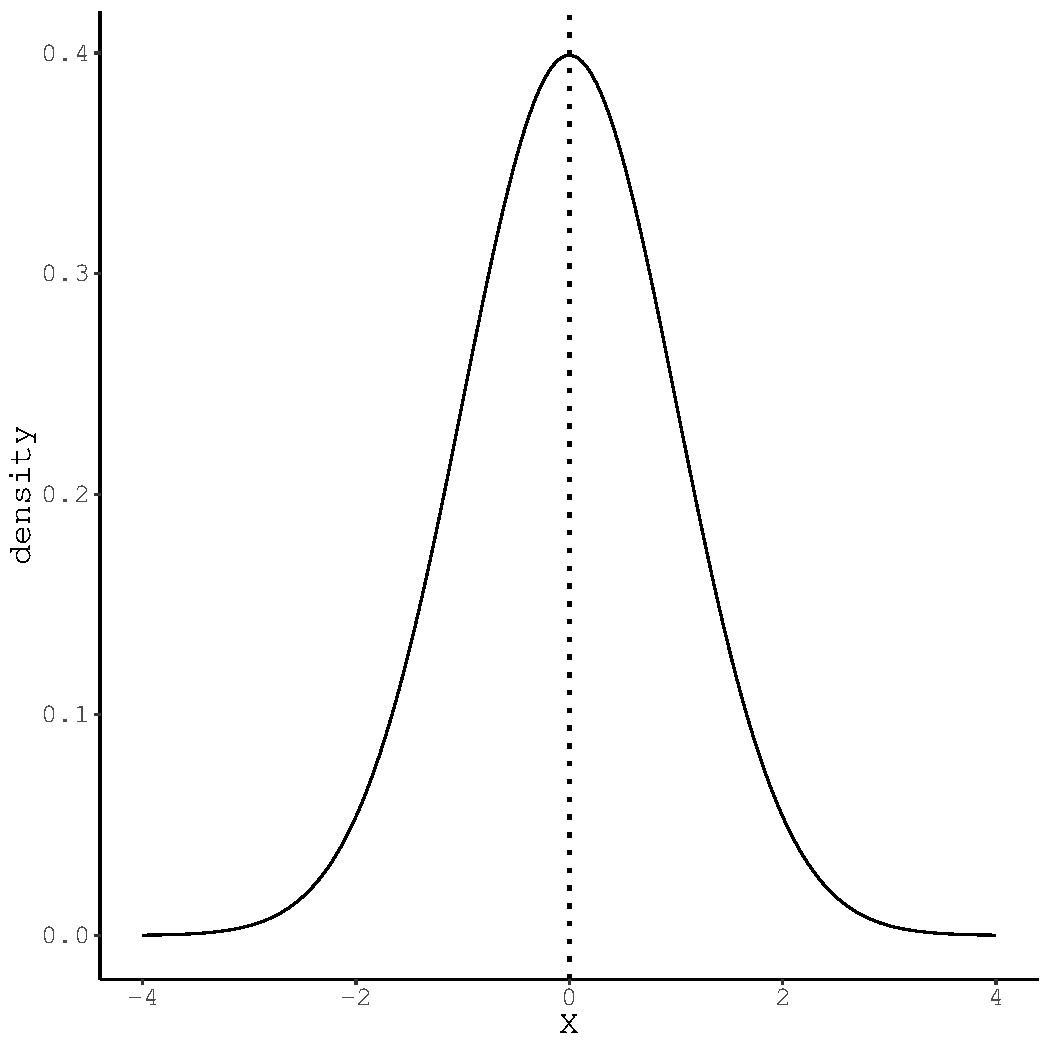
\includegraphics[width=\maxwidth]{figure/unnamed-chunk-1-1} 

}


\end{knitrout}

\end{column}
\end{columns}

\end{frame}

%------------------------------------------------------------------------------%

\begin{frame}{Flavors of Probability Distribution}

  \begin{columns}
    \begin{column}{0.5\textwidth}
      The distributions we consider in regression problems have
      \emph{conditional means}.
      \vb
      \begin{itemize}
      \item The value of $Y$ that we expect for each observation is defined by
        the observations' individual characteristics.
        \vb
      \item This type of distribution is called ``conditional.''
      \end{itemize}
    \end{column}

    \begin{column}{0.5\textwidth}

      \begin{figure}
        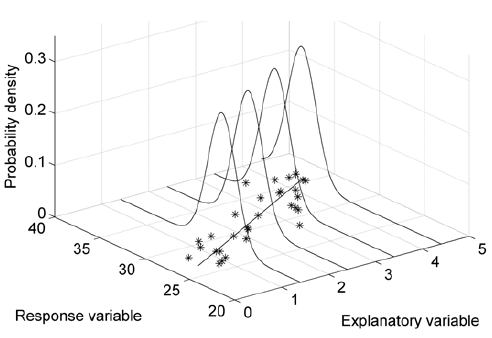
\includegraphics[width = \textwidth]{%
          figures/conditional_density_figure.png%
        }\\
        \va
        \tiny{Image retrieved from:
            \url{http://www.seaturtle.org/mtn/archives/mtn122/mtn122p1.shtml}}
      \end{figure}

    \end{column}
  \end{columns}

\end{frame}

%------------------------------------------------------------------------------%

\begin{frame}{Flavors of Probability Distribution}

  \begin{columns}
    \begin{column}{0.5\textwidth}
      Even a simple comparison of means implies a conditional distribution.
      \vb
      \begin{itemize}
      \item The solid curve corresponds to outcome values for one group.
        \vb
      \item The dashed curve represents outcomes from the other group.
      \end{itemize}
    \end{column}

    \begin{column}{0.5\textwidth}


\begin{knitrout}\footnotesize
\definecolor{shadecolor}{rgb}{0.878, 0.918, 0.933}\color{fgcolor}

{\centering 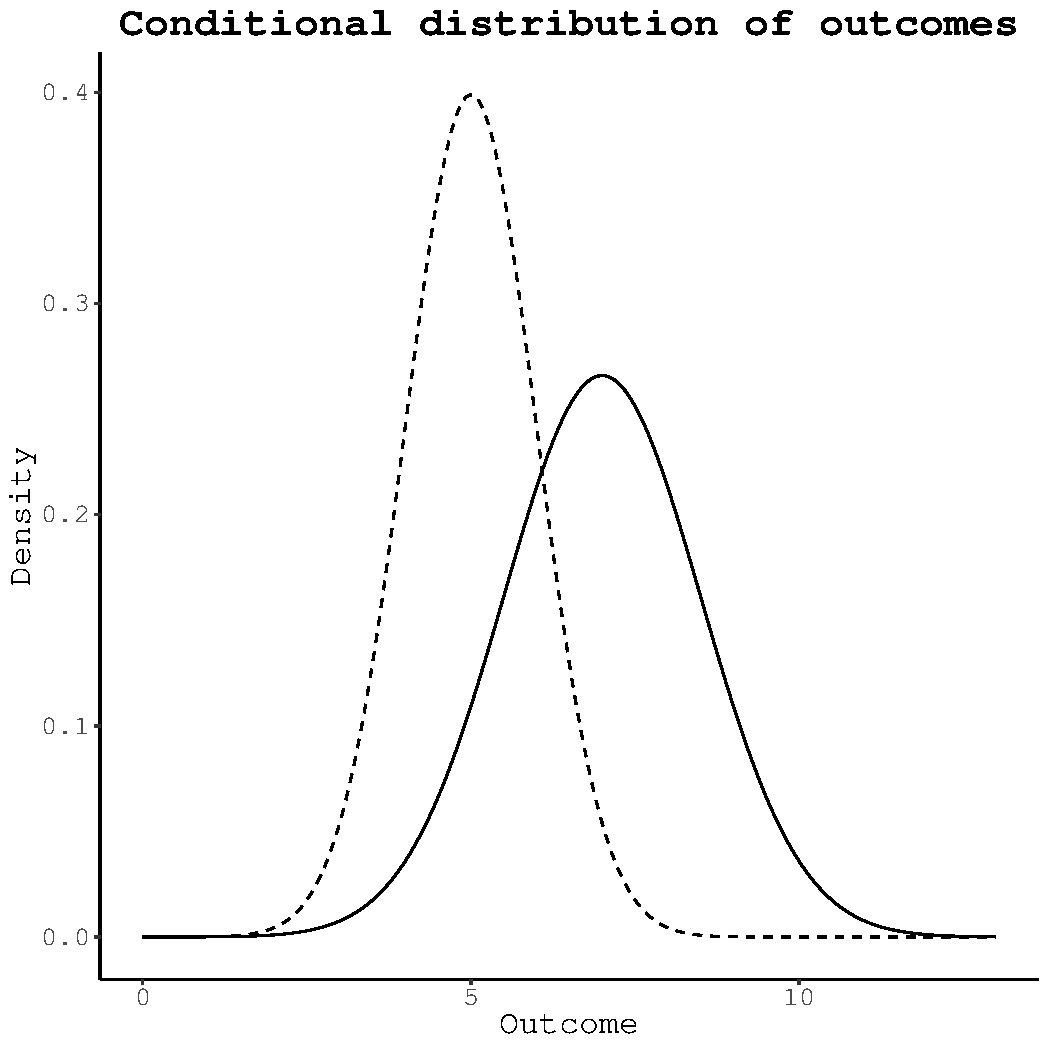
\includegraphics[width=\maxwidth]{figure/unnamed-chunk-2-1} 

}


\end{knitrout}

\end{column}
\end{columns}

\end{frame}

%------------------------------------------------------------------------------%

\begin{frame}{Projecting a Distribution onto the Plane}

  \begin{columns}
    \begin{column}{0.5\textwidth}
      In practice, we only interact with the X-Y plane of the previous 3D
      figure.
      \vb
      \begin{itemize}
      \item On the Y-axis, we plot our outcome variable
        \vb
      \item The X-axis represents the predictor variable upon which we condition
        the mean of $Y$.
      \end{itemize}
    \end{column}

    \begin{column}{0.5\textwidth}

\begin{knitrout}\footnotesize
\definecolor{shadecolor}{rgb}{0.878, 0.918, 0.933}\color{fgcolor}

{\centering 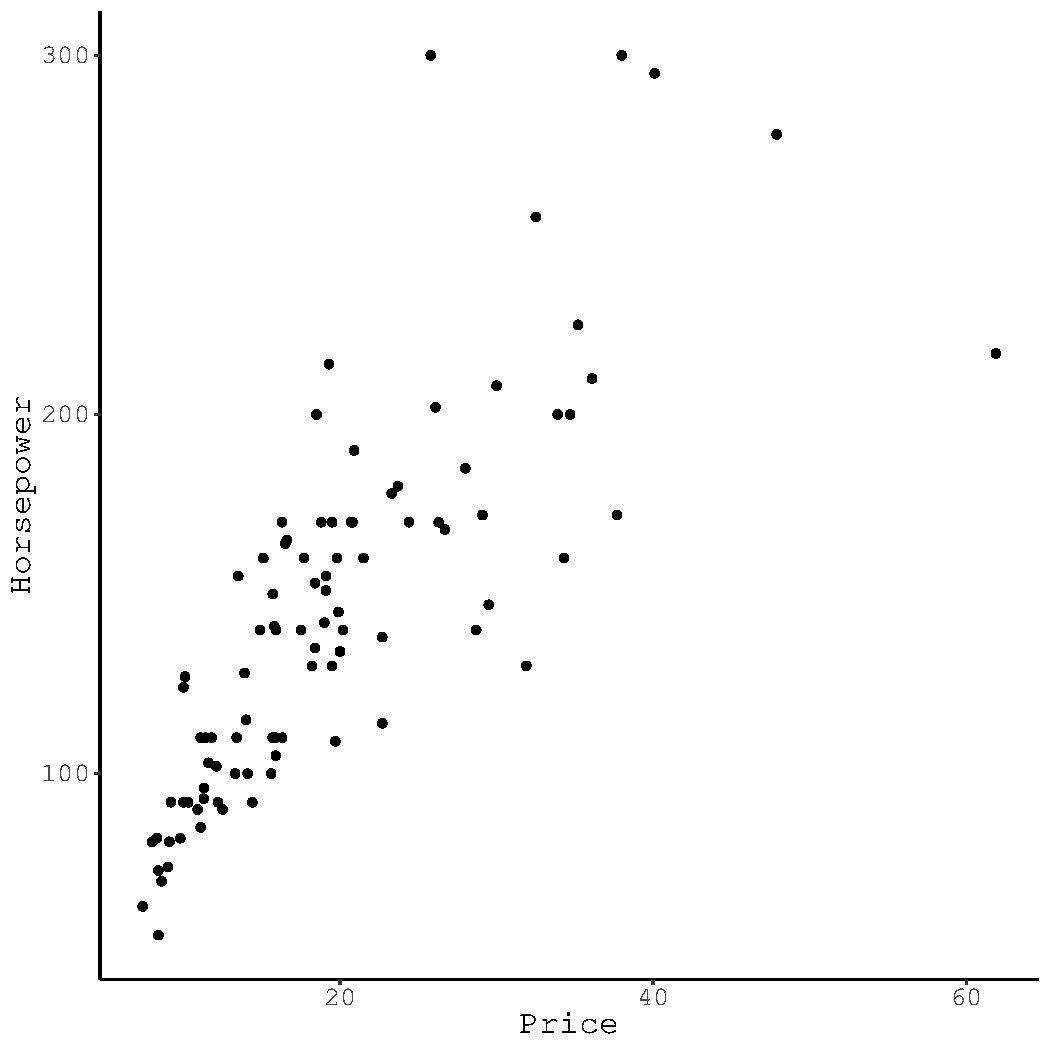
\includegraphics[width=\maxwidth]{figure/unnamed-chunk-3-1} 

}


\end{knitrout}

\end{column}
\end{columns}

\end{frame}

%------------------------------------------------------------------------------%

\begin{frame}{Modeling the X-Y Relationship in the Plane}

  \begin{columns}
    \begin{column}{0.5\textwidth}
      We want to explain the relationship between $Y$ and $X$ by finding the
      line that traverses the scatterplot as ``closely'' as possible to each
      point.
      \vb
      \begin{itemize}
      \item This is the ``best fit line''.
        \vb
      \item For any given value of $X$ the corresponding point on the best fit
        line is our best guess for the value of $Y$, given the model.
      \end{itemize}
    \end{column}

    \begin{column}{0.5\textwidth}

\begin{knitrout}\footnotesize
\definecolor{shadecolor}{rgb}{0.878, 0.918, 0.933}\color{fgcolor}

{\centering 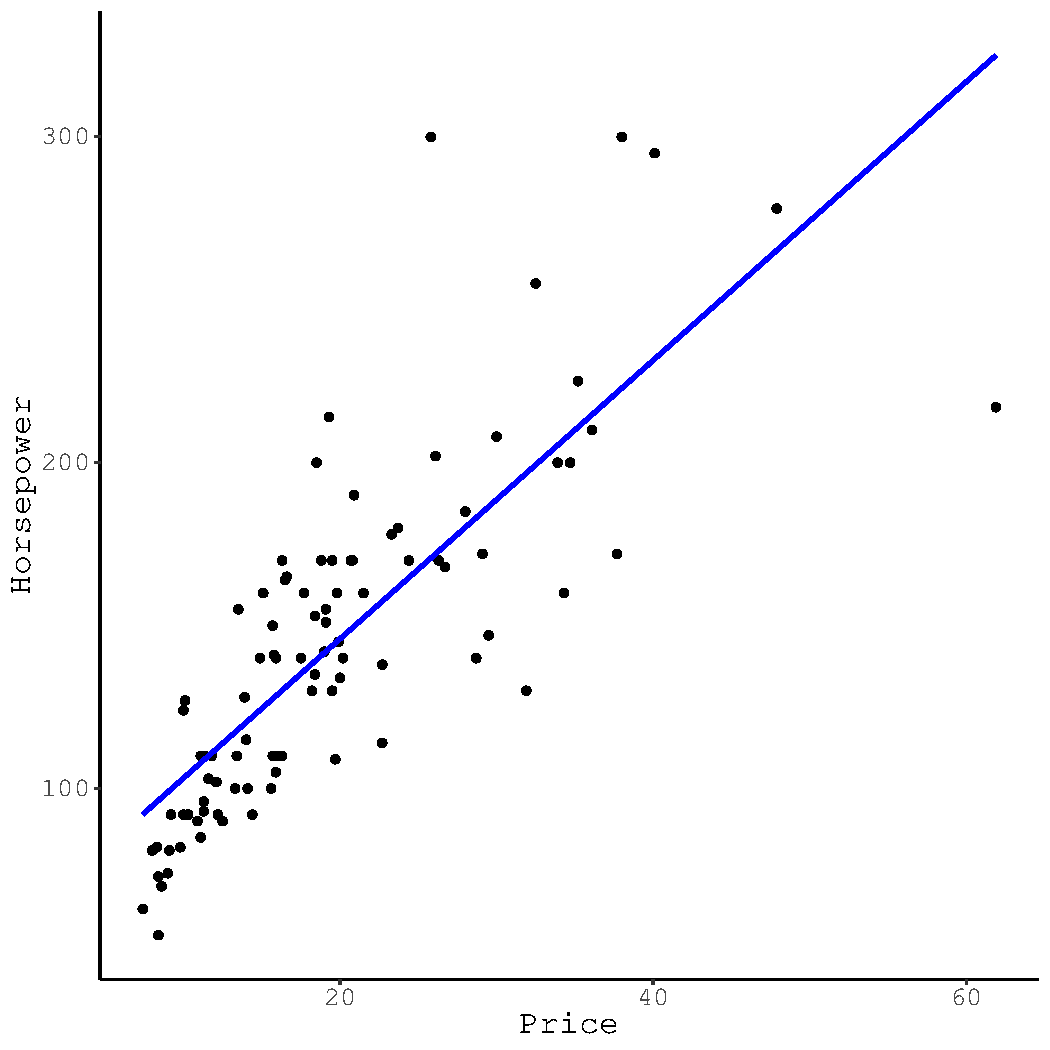
\includegraphics[width=\maxwidth]{figure/unnamed-chunk-4-1} 

}


\end{knitrout}

\end{column}
\end{columns}

\end{frame}

\watermarkon %-----------------------------------------------------------------%

\sectionslide{Simple Linear Regression}

%------------------------------------------------------------------------------%

\begin{frame}{Simple Linear Regression}

  The best fit line is defined by a simple equation:
  \begin{align*}
    \hat{Y} = \hat{\beta}_0 + \hat{\beta}_1 X
  \end{align*}
  The above should look very familiar:
  \begin{align*}
    Y &= m X + b\\
      &= \hat{\beta}_1 X + \hat{\beta}_0
  \end{align*}
  $\hat{\beta}_0$ is the \emph{intercept}.
  \begin{itemize}
  \item The $\hat{Y}$ value when $X = 0$.
  \item The expected value of $Y$ when $X = 0$.
  \end{itemize}
  \vb
  $\hat{\beta}_1$ is the \emph{slope}.
  \begin{itemize}
  \item The change in $\hat{Y}$ for a unit change in $X$.
  \item The expected change in $Y$ for a unit change in $X$.
  \end{itemize}

\end{frame}

\watermarkoff %----------------------------------------------------------------%

\begin{frame}{Thinking about Error}

  \begin{columns}[T]
    \begin{column}{0.5\textwidth}
      The equation $\hat{Y} = \hat{\beta}_0 + \hat{\beta}_1 X$ only describes
      the best fit line.
      \begin{itemize}
      \item It does not fully quantify the relationship between $Y$ and $X$.\\
      \end{itemize}
      \vb
      \only<2>{
        We still need to account for the estimation error.
        \begin{align*}
          Y = {\color{blue}\hat{\beta}_0 + \hat{\beta}_1 X} + {\color{red}\hat{\varepsilon}}
        \end{align*}
      }
    \end{column}

    \begin{column}{0.5\textwidth}

      \only<1>{
\begin{knitrout}\footnotesize
\definecolor{shadecolor}{rgb}{0.878, 0.918, 0.933}\color{fgcolor}

{\centering 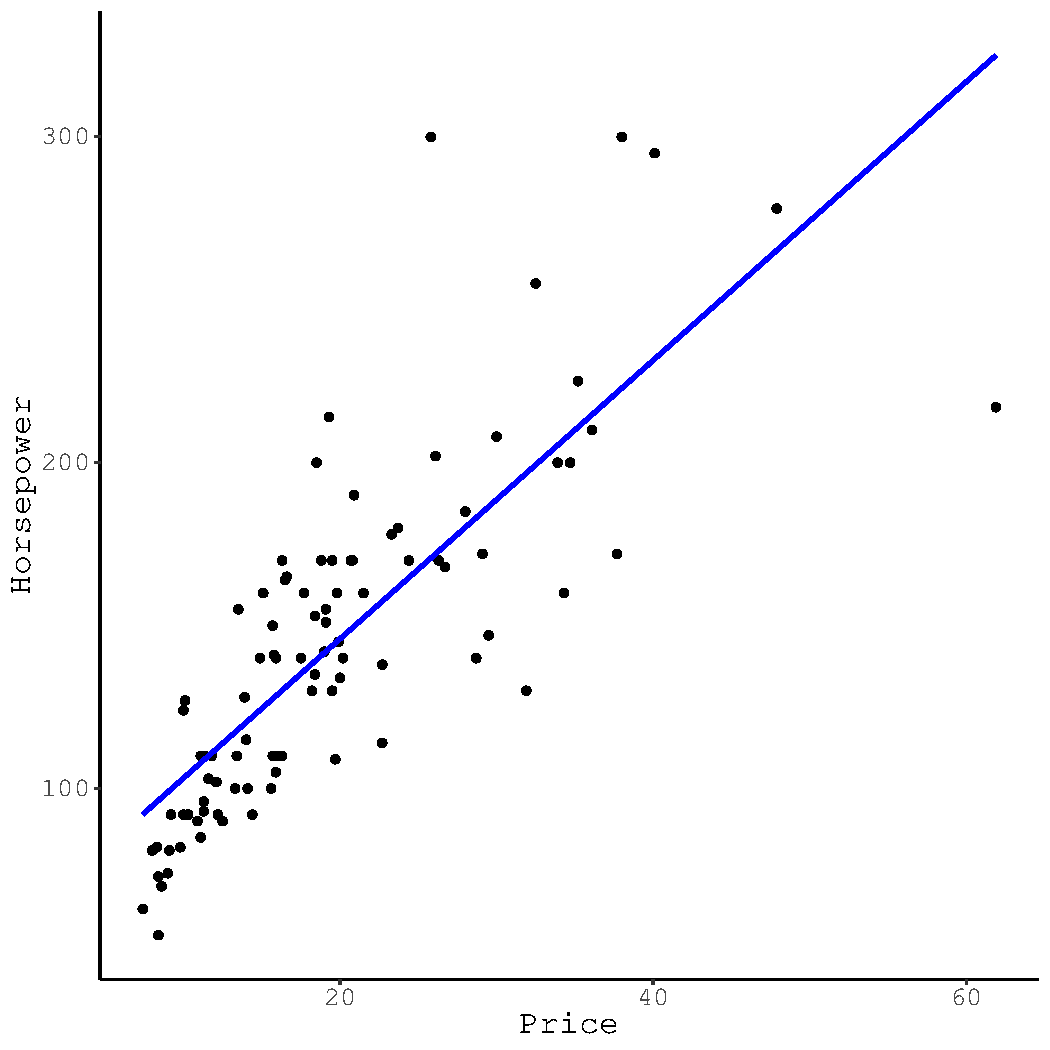
\includegraphics[width=\maxwidth]{figure/unnamed-chunk-5-1} 

}


\end{knitrout}
      }
      \only<2>{

\begin{knitrout}\footnotesize
\definecolor{shadecolor}{rgb}{0.878, 0.918, 0.933}\color{fgcolor}

{\centering 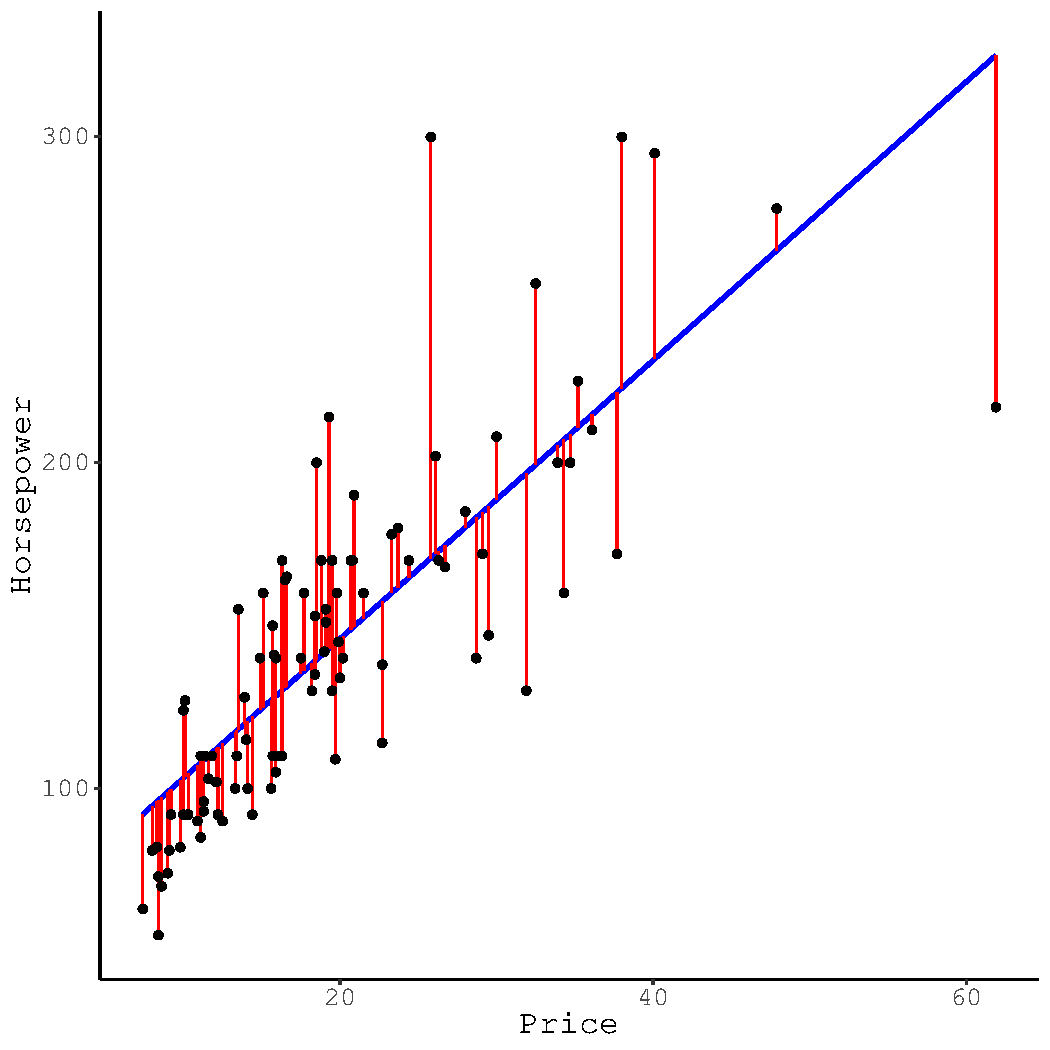
\includegraphics[width=\maxwidth]{figure/unnamed-chunk-6-1} 

}


\end{knitrout}
      }

    \end{column}
  \end{columns}

\end{frame}

\watermarkon %-----------------------------------------------------------------%

\begin{frame}{Estimating the Regression Coefficients}

  The purpose of regression analysis is to use a sample of $N$ observed $\{Y_n,
  X_n\}$ pairs to find the best fit line defined by $\hat{\beta}_0$ and
  $\hat{\beta}_1$.
  \vb
  \begin{itemize}
  \item The most popular method of finding the best fit line involves minimizing
    the sum of the squared residuals.
    \vb
  \item $RSS = \sum_{n = 1}^N \hat{\varepsilon}_n^2$
  \end{itemize}

\end{frame}

\watermarkoff %----------------------------------------------------------------%

\begin{frame}{Residuals as the Basis of Estimation}

  \begin{columns}
    \begin{column}{0.5\textwidth}

      The $\hat{\varepsilon}_n$ are defined in terms of deviations between each
      observed $Y_n$ value and the corresponding $\hat{Y}_n$.
      \begin{align*}
        \hat{\varepsilon}_n = Y_n - \hat{Y}_n =
        Y_n - \left(\hat{\beta}_0 + \hat{\beta}_1 X_n\right)
      \end{align*}
      Each $\hat{\varepsilon}_n$ is squared before summing to remove negative
      values.
      \begin{align*}
        RSS &= \sum_{n = 1}^N \hat{\varepsilon}_n^2 =
              \sum_{n = 1}^N \left(Y_n - \hat{Y}_n\right)^2\\
            &= \sum_{n = 1}^N \left(Y_n - \hat{\beta}_0 - \hat{\beta}_1
              X_n\right)^2
      \end{align*}
    \end{column}

    \begin{column}{0.5\textwidth}

\begin{knitrout}\footnotesize
\definecolor{shadecolor}{rgb}{0.878, 0.918, 0.933}\color{fgcolor}

{\centering 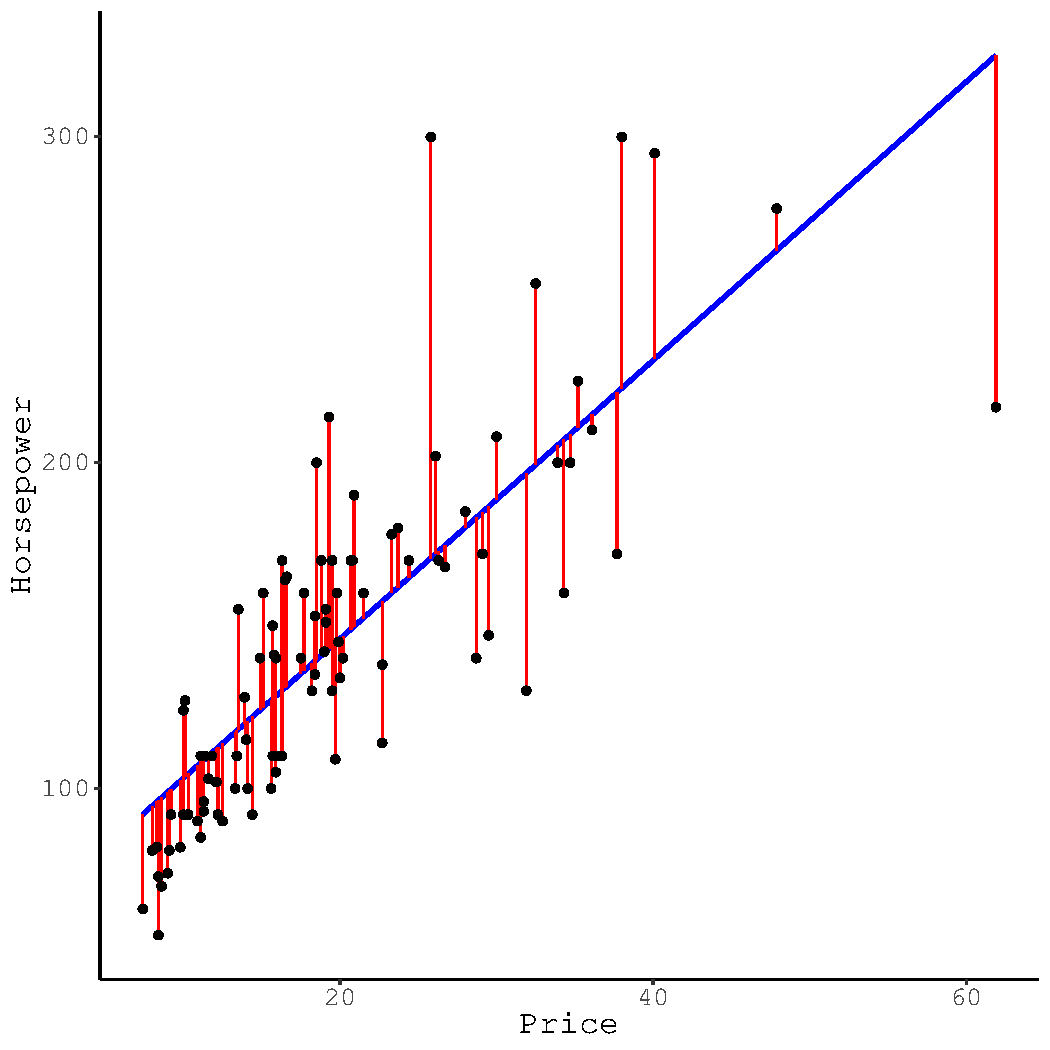
\includegraphics[width=\maxwidth]{figure/unnamed-chunk-7-1} 

}


\end{knitrout}

\end{column}
\end{columns}

\end{frame}

\watermarkon %-----------------------------------------------------------------%

\begin{frame}[fragile]{Least Squares Example}

  Estimate the least squares coefficients for our example data:

\begin{knitrout}\footnotesize
\definecolor{shadecolor}{rgb}{0.878, 0.918, 0.933}\color{fgcolor}\begin{kframe}
\begin{alltt}
\hlcom{#data(Cars93)}
\hlstd{out1} \hlkwb{<-} \hlkwd{lm}\hlstd{(Horsepower} \hlopt{~} \hlstd{Price,} \hlkwc{data} \hlstd{= Cars93)}
\hlkwd{coef}\hlstd{(out1)}
\end{alltt}
\begin{verbatim}
## (Intercept)       Price 
##   60.447578    4.273796
\end{verbatim}
\end{kframe}
\end{knitrout}



The estimated intercept is $\hat{\beta}_0 = 60.45$.
\begin{itemize}
\item A free car is expected to have 60.45 horsepower.
\end{itemize}
\vb
The estimated slope is: $\hat{\beta}_1 = 4.27$.
\begin{itemize}
\item For every additional \$1000 in price, a car is expected to gain 4.27
  horsepower.
\end{itemize}

\end{frame}

%------------------------------------------------------------------------------%

\sectionslide{Inference for Linear Models}

\watermarkoff %----------------------------------------------------------------%

\begin{frame}[shrink = 5]{Sampling Distribution}

  A sampling distribution is simply the probability distribution of a parameter.

  \begin{columns}
    \begin{column}{0.5\textwidth}

      \begin{itemize}
      \item The \emph{population} is defined by an infinite sequence of repeated
        estimations.
        \vb
        \begin{itemize}
        \item The sampling distribution quantifies the possible values of the
          statistic over infinite repeated sampling.
        \end{itemize}
        \vb
      \item The area of a region under the curve represents the probability of
        observing a \emph{statistic} within the corresponding interval.
      \end{itemize}

    \end{column}
    \begin{column}{0.5\textwidth}

\begin{knitrout}\footnotesize
\definecolor{shadecolor}{rgb}{0.878, 0.918, 0.933}\color{fgcolor}

{\centering 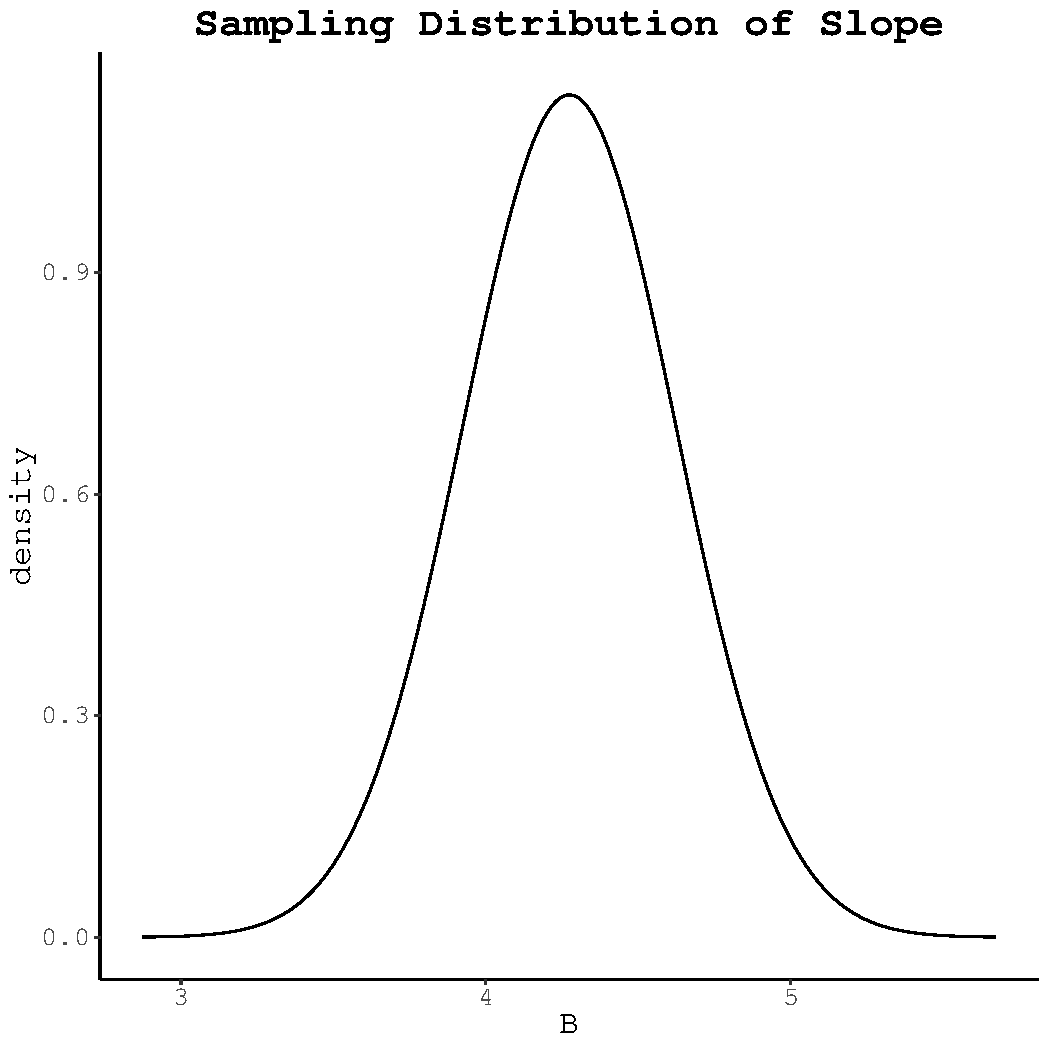
\includegraphics[width=\maxwidth]{figure/unnamed-chunk-10-1} 

}


\end{knitrout}

\end{column}
\end{columns}

\textsc{Some Intuition}: \url{http://onlinestatbook.com/stat_sim/sampling_dist/}

\end{frame}

\watermarkon %-----------------------------------------------------------------%

\begin{frame}{Test Statistics}
 
  To ``test'' a slope coefficient, $\hat{\beta}$, we need a point of comparison.
  \begin{itemize}
  \item The \emph{null-hypothesized} value of the slope, 
    $H_0: \beta = \tilde{\beta}$.
  \end{itemize}
  
  \vb
  
  Our hypothesis test is actually a test for the size of the difference:
  $\hat{\beta} - \tilde{\beta}$
  \begin{itemize}
  \item We define a \emph{test statistic}, $t$, to quantify the size of this 
    difference accounting for the precision with which we've estimated 
    $\hat{\beta}$.
  \end{itemize}
  
  \vb
  
  We can construct the test statistic for $\hat{\beta}$ as follows:
  \begin{align*}
    t = \frac{\hat{\beta} - \tilde{\beta}}{SE\left(\hat{\beta}\right)} 
    ~~\overset{\tilde{\beta} = 0}{\mathlarger{\Rightarrow}}~~
    t = \frac{\hat{\beta} - 0}{SE\left(\hat{\beta}\right)} = 
    \frac{\hat{\beta}}{SE\left(\hat{\beta}\right)}
  \end{align*}
  


For the slope in our example, we get a test statistic of:
\begin{align*}
  t = \frac{\hat{\beta}_1}{SE\left(\hat{\beta}_1\right)} = 
    \frac{4.27}{0.35} = 12.2
\end{align*}

\end{frame}

\watermarkoff %----------------------------------------------------------------%

\begin{frame}[shrink = 5]{Sampling Distribution of Test Statistic}

 \begin{columns}
   \begin{column}{0.5\textwidth}
     
     The t-statistic also has a sampling distribution.
     \vc
     \begin{itemize}
     \item Quantifies the possible values we could get if we repeatedly drew
       samples, of the \underline{same size}, from the \underline{same 
         population} and re-computed a t-statistic each time.
     \vb
     \item The distribution under the null hypothesis assumes a population 
       wherein $\hat{\beta}$ = $\tilde{\beta}$, and, consequently, $t = 0$.
     \end{itemize}
     
   \end{column}
   \begin{column}{0.5\textwidth}
     
\begin{knitrout}\footnotesize
\definecolor{shadecolor}{rgb}{0.878, 0.918, 0.933}\color{fgcolor}

{\centering 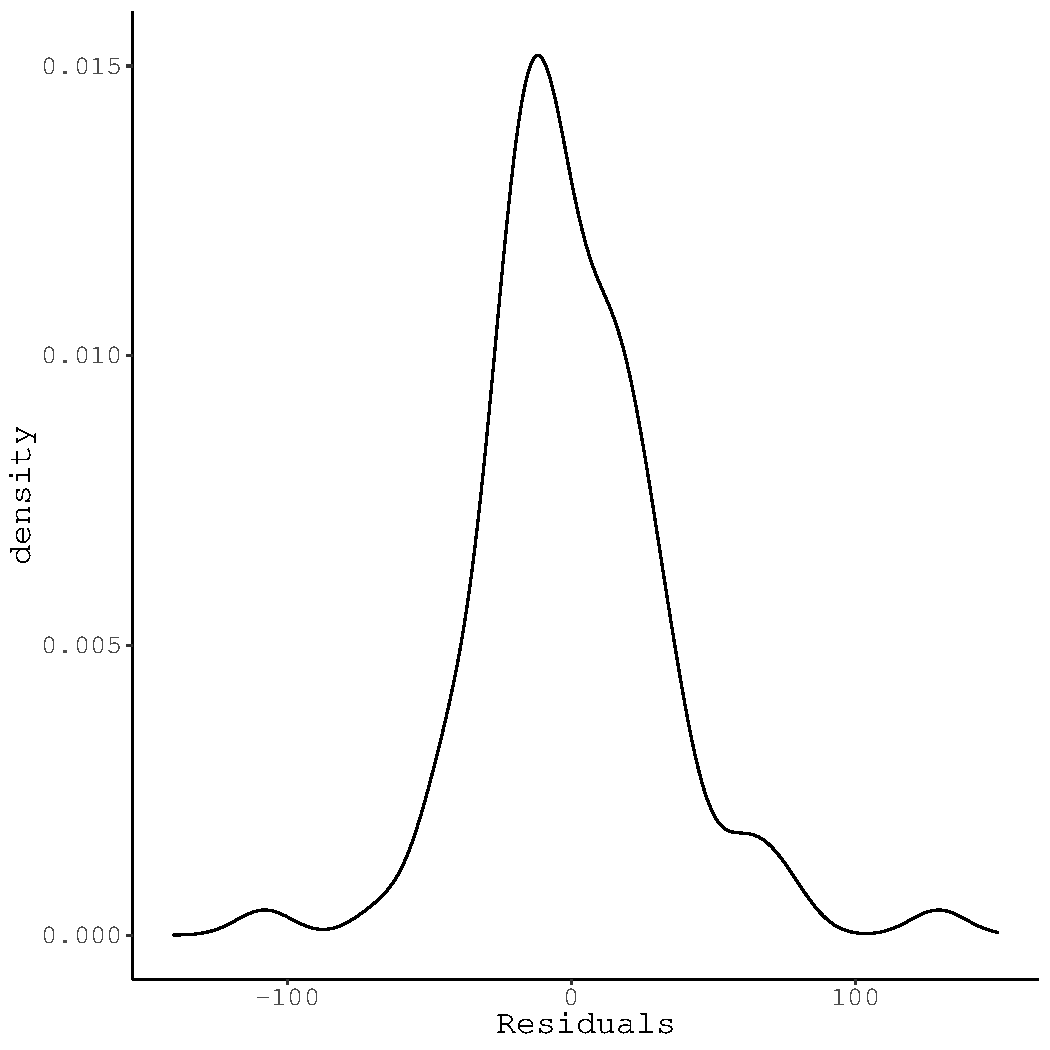
\includegraphics[width=\maxwidth]{figure/unnamed-chunk-12-1} 

}


\end{knitrout}

   \end{column}
 \end{columns}
 
\end{frame}
\watermarkon %-----------------------------------------------------------------%

\begin{frame}{P-Values}

  Once we compute our estimated test statistic, $\hat{t}$, we compare it to the
  appropriate null-hypothesized sampling distribution.
  \vb
  \begin{itemize}
    \item By calculating the area in the null distribution that exceeds our
      estimated test statistic, we can compute the probability of observing the
      given test statistic, or one more extreme, if the null hypothesis were
      true.  
      \vb
      \begin{itemize}
      \item In other words, we can compute the probability of having sampled the
        data we observed, or more unusual data, from a population wherein there
        is no true difference between $\hat{\beta}$ and $\tilde{\beta}$.
      \end{itemize}
      \vb
    \item This value is the infamous \emph{p-value}.
  \end{itemize}
  
\end{frame}

\watermarkoff %----------------------------------------------------------------%

\begin{frame}[fragile]{P-Values}

  \begin{columns}
    \begin{column}{0.5\textwidth}

\begin{knitrout}\footnotesize
\definecolor{shadecolor}{rgb}{0.878, 0.918, 0.933}\color{fgcolor}

{\centering 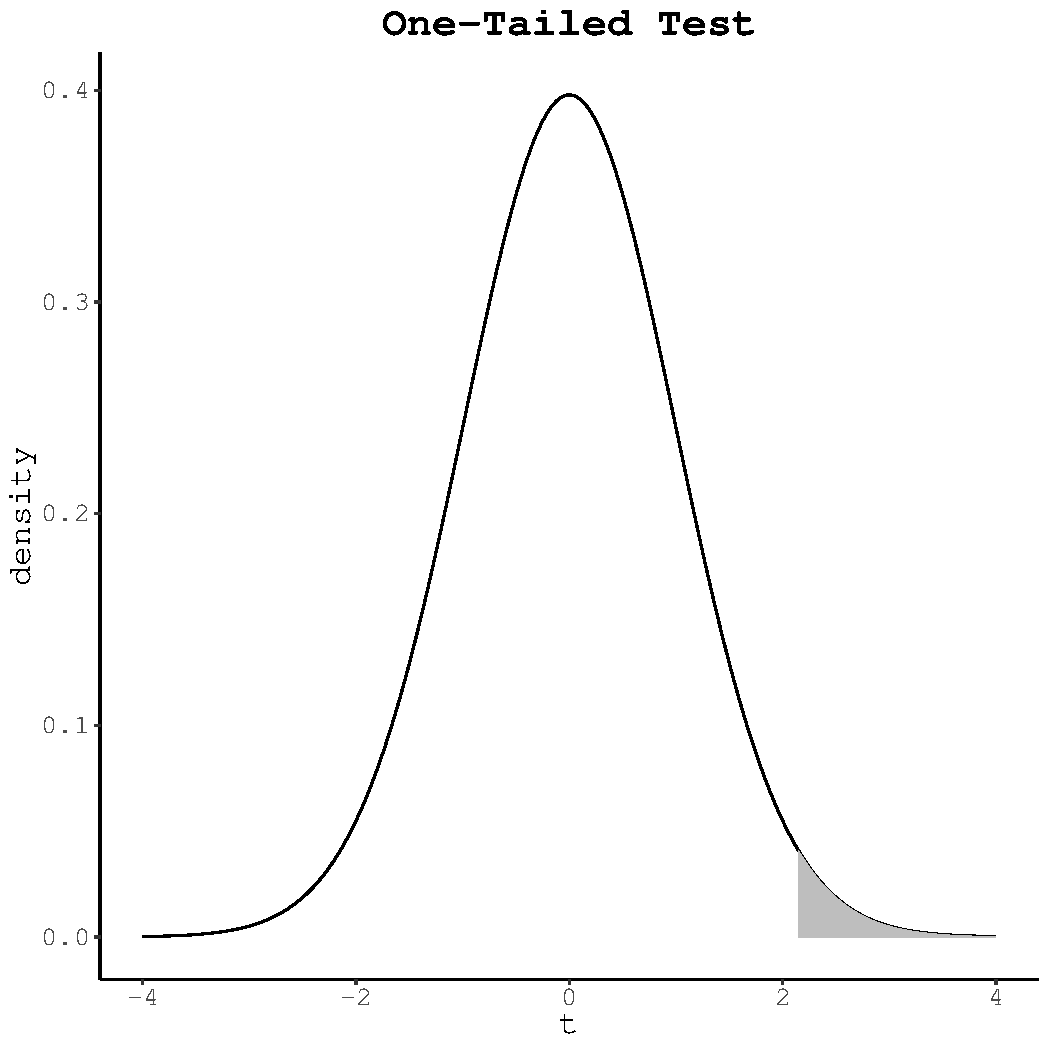
\includegraphics[width=\maxwidth]{figure/unnamed-chunk-13-1} 

}


\end{knitrout}

    \end{column}
    \begin{column}{0.5\textwidth}
     
\begin{knitrout}\footnotesize
\definecolor{shadecolor}{rgb}{0.878, 0.918, 0.933}\color{fgcolor}

{\centering 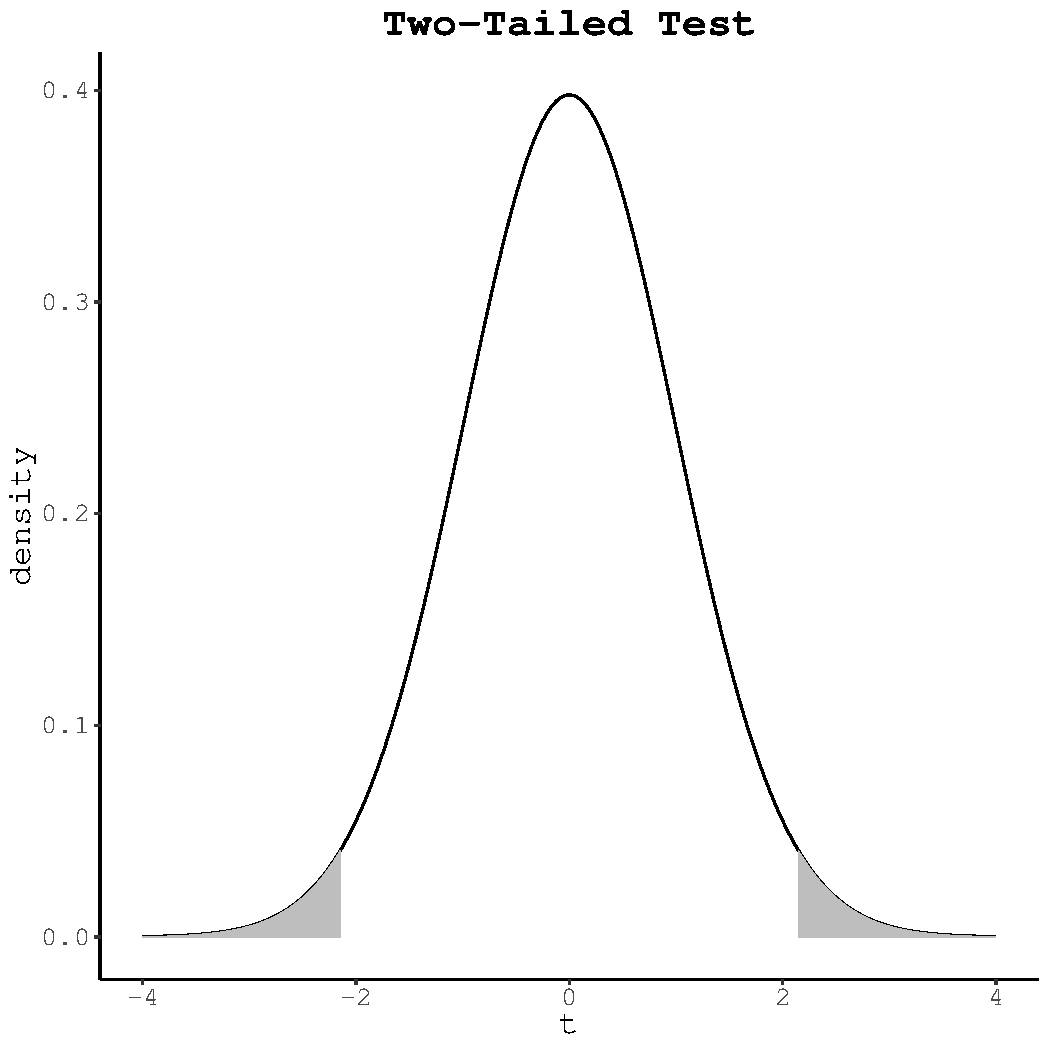
\includegraphics[width=\maxwidth]{figure/unnamed-chunk-14-1} 

}


\end{knitrout}

    \end{column}
  \end{columns}

\end{frame}

\watermarkon %-----------------------------------------------------------------%

\begin{frame}{Interpreting P-Values}



Consider the one-tailed test for our estimated test-statistic of $\hat{t} =
2.15$ that produces a p-value of $p = 0.017$.
\vc
\begin{itemize}
\item We \emph{\underline{cannot}} say that there is a $0.017$
  probability that the true mean difference is greater than zero.
  \vc
\item We \emph{\underline{cannot}} say that there is a $0.017$
  probability that the alternative hypothesis is true.
  \vc
\item We \emph{\underline{cannot}} say that there is a $0.017$
  probability that the null hypothesis is false.
  \vc
\item We \emph{\underline{cannot}} say that there is a $0.017$
  probability that the observed result is due to chance alone.
  \vc
\item We \emph{\underline{cannot}} say that there is a $0.017$
  probability of replicating the observed effect in future studies.
\end{itemize}

\end{frame}

\watermarkoff %----------------------------------------------------------------%

\begin{frame}{Interpreting P-Values}
  
  \begin{columns}
    \begin{column}{0.5\textwidth}
      
      The p-value tells us $P(t \geq \hat{t}|H_0)$
      \begin{itemize}
      \item What we really want to know is $P(H_0|t \geq \hat{t})$.
      \end{itemize}
      \vb 
      All that we \emph{\underline{can}} say is that there is a
      $0.017$ probability of observing a test statistic
      at least as large as $\hat{t}$, if the null hypothesis is true.
      \vc
      \begin{itemize}
      \item Our test uses the same logic as \emph{proof by contradiction}.
      \end{itemize}
      
    \end{column}
    \begin{column}{0.5\textwidth}

\begin{knitrout}\footnotesize
\definecolor{shadecolor}{rgb}{0.878, 0.918, 0.933}\color{fgcolor}

{\centering 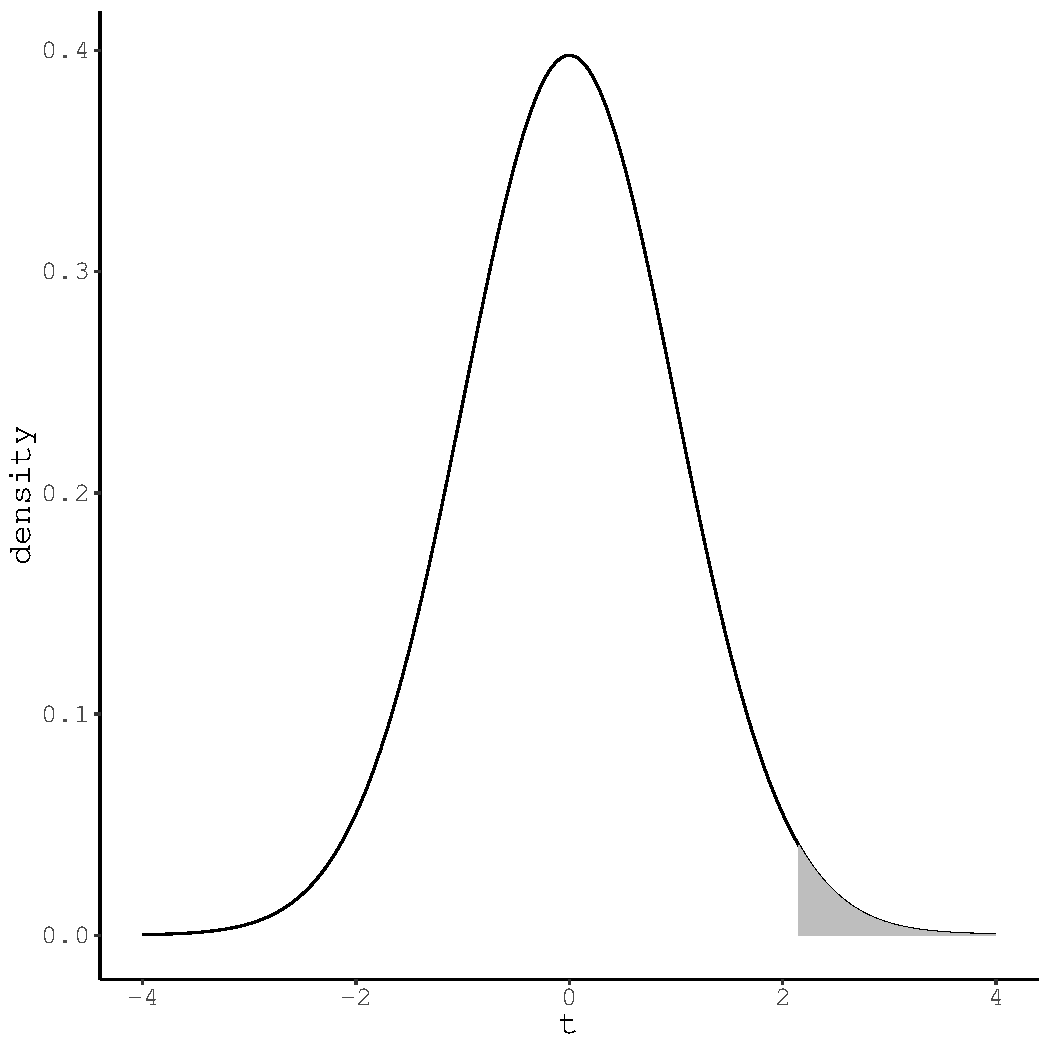
\includegraphics[width=\maxwidth]{figure/unnamed-chunk-16-1} 

}


\end{knitrout}

    \end{column}
  \end{columns}

\end{frame}

%------------------------------------------------------------------------------%

\comment{%%%%%%%%%%%%%%%%%%%%%%%%%%%%%%%%%%%%%%%%%%%%%%%%%%%%%%%%%%%%%%%%%%%%%%%
\begin{frame}{Interpreting P-Values}

\begin{columns}
  \begin{column}{0.5\textwidth}

    Note that $P(t \geq \hat{t}|H_0) \neq P(t = \hat{t}|H_0)$
    \begin{itemize}
    \item We \emph{\underline{cannot}} say that there is a
      $0.017$ probability of observing $\hat{t}$, if the null
      hypothesis is true.
    \end{itemize}
    \vb
    The probability of observing any individual point on a continuous
    distribution is exactly zero.
    \vc
    \begin{itemize}
    \item $P(t = \hat{t}|H_0) = 0$
    \end{itemize}

  \end{column}
  \begin{column}{0.5\textwidth}

\begin{knitrout}\footnotesize
\definecolor{shadecolor}{rgb}{0.878, 0.918, 0.933}\color{fgcolor}

{\centering 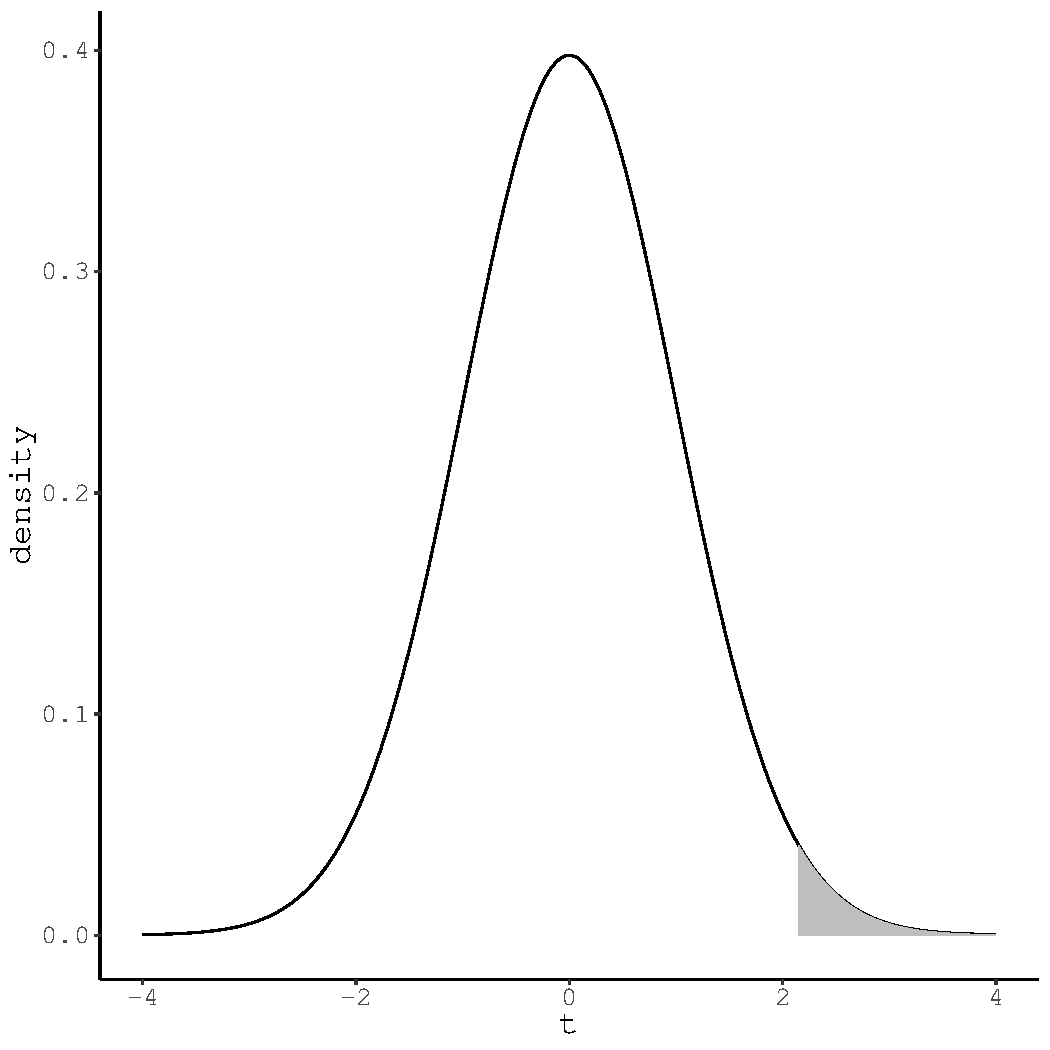
\includegraphics[width=\maxwidth]{figure/unnamed-chunk-17-1} 

}


\end{knitrout}

\end{column}
\end{columns}

\end{frame}
}%%%%%%%%%%%%%%%%%%%%%%%%%%%%%%%%%%%%%%%%%%%%%%%%%%%%%%%%%%%%%%%%%%%%%%%%%%%%%%%

\watermarkon %-----------------------------------------------------------------%

\begin{frame}{Inferential Tools: Confidence Intervals}

  We can also construct confidence intervals by:
  \begin{align*}
    CI = \hat{\beta} \pm t_{crit} \times SE\left(\hat{\beta}\right)
  \end{align*}
  
  For our example slope, we get a 95\% CI of:
  \begin{align*}
    CI_{95} = 4.27 \pm 1.99 \times
    0.35 = [3.57; 4.97]
  \end{align*}
  Which suggests that we can be 95\% certain that the true value of $\beta_1$ is
  somewhere between $3.57$ and $4.97$.
  \vc
  \begin{itemize}
  \item We are \emph{95\% certain} in the sense that if we repeat this analysis 
    an infinite number of times, 95\% of the CIs that we calculate will surround
    the true value of $\beta_1$.
  \end{itemize}
  
\end{frame}

%------------------------------------------------------------------------------%

\begin{frame}{Interpreting Confidence Intervals}
  
  Say we estimate a regression slope of $\hat{\beta}_1 = 0.5$ with an associated
  95\% confidence interval of $CI = [0.25; 0.75]$.
  \pause
  \vc
  \begin{itemize}
  \item We \emph{\underline{cannot}} say that there is 95\% chance that the true 
    value of $\beta_1$ is between 0.25 and 0.75.
    \vc
  \item We \emph{\underline{cannot}} say that the true value of $\beta_1$ is 
    between 0.25 and 0.75, with probability 0.95.
  \end{itemize}
  \vb  
  \pause
  The true value of $\beta_1$ is fixed; it's a single quantity.
  \begin{itemize}
  \item $\beta_1$ is either in our estimated interval or it is not; there is no 
    uncertainty.
    \vc
  \item The probability that $\beta_1$ is within our estimated interval is either 
    exactly 1 or exactly 0.
  \end{itemize}
  
\end{frame}

\watermarkoff %----------------------------------------------------------------%

\begin{frame}{Interpreting Confidence Intervals}
  
  We don't talk about 95\% probabilities when interpreting CIs; instead, we 
  talk about 95\% confidence.
  \vc
  \begin{columns}
    \begin{column}{0.5\textwidth}
      
      \begin{itemize}
      \item If we collected a new sample---of the same size---re-estimated our 
        model, and re-computed the 95\% CI for $\hat{\beta_1}$, we would get a 
        different interval.
        \vc
      \item Repeating this process an infinite number of times would give us a 
        distribution of CIs.
        \vc
      \item 95\% of those CIs would surround the true value of $\beta_1$.
      \end{itemize}
      
    \end{column}
    \begin{column}{0.5\textwidth}
      
\begin{knitrout}\footnotesize
\definecolor{shadecolor}{rgb}{0.878, 0.918, 0.933}\color{fgcolor}

{\centering 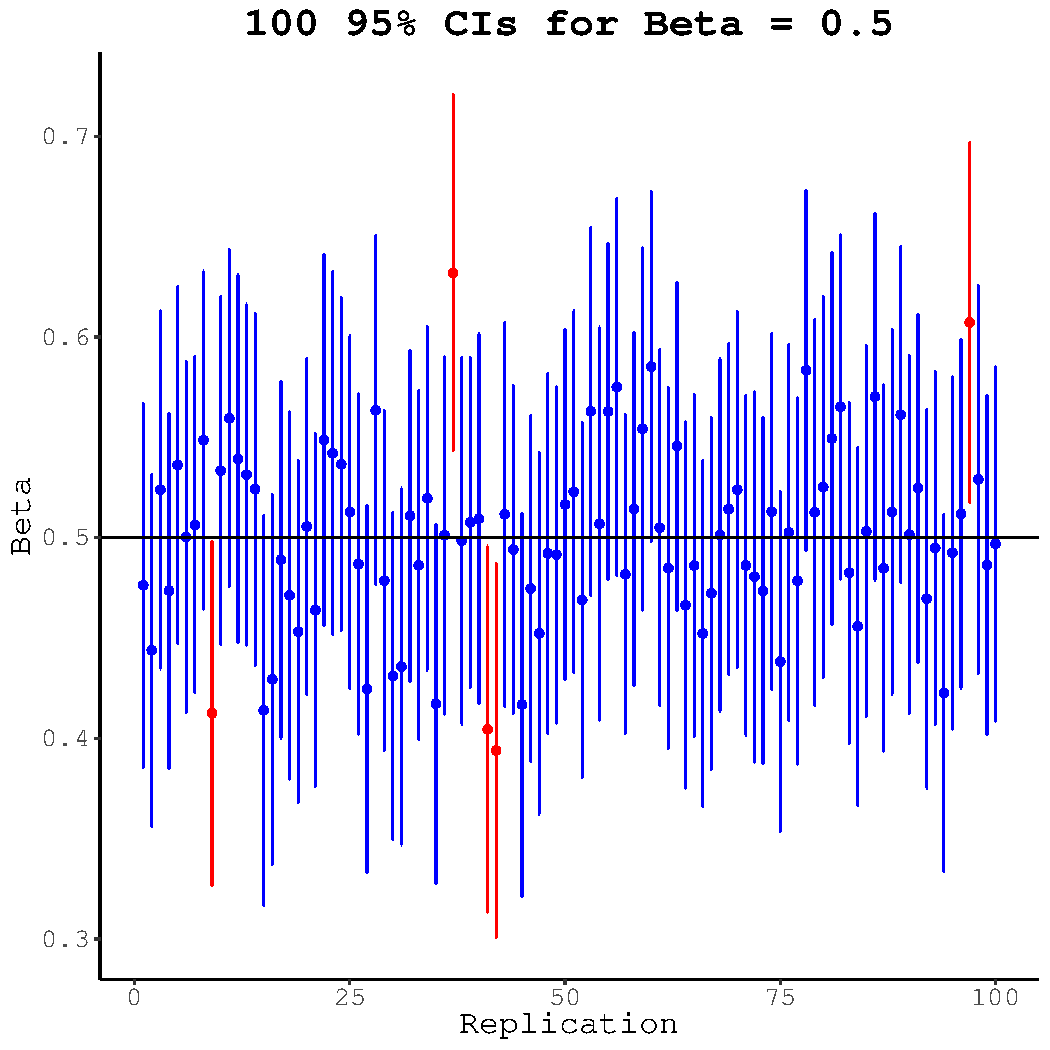
\includegraphics[width=\maxwidth]{figure/unnamed-chunk-18-1} 

}


\end{knitrout}

\end{column}
\end{columns}

\end{frame}

%------------------------------------------------------------------------------%

\comment{%%%%%%%%%%%%%%%%%%%%%%%%%%%%%%%%%%%%%%%%%%%%%%%%%%%%%%%%%%%%%%%%%%%%%%%
\begin{frame}{Inference with Confidence Intervals}
  
  In terms of sampling distributions, our inferential task is to say something 
  about how distinct the null and alternative distributions are.
 


\begin{columns}
  \begin{column}{0.5\textwidth}
   
\begin{knitrout}\footnotesize
\definecolor{shadecolor}{rgb}{0.878, 0.918, 0.933}\color{fgcolor}

{\centering 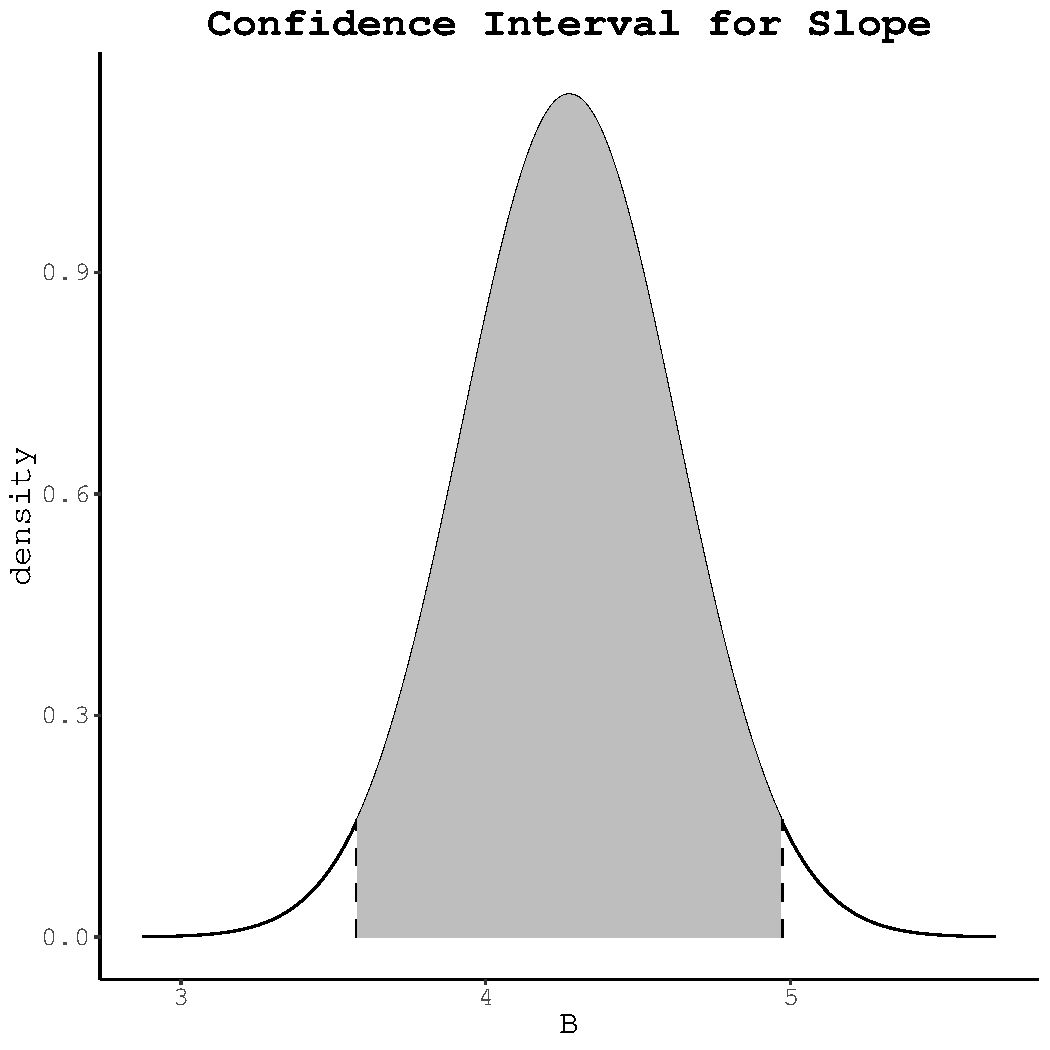
\includegraphics[width=\maxwidth]{figure/unnamed-chunk-20-1} 

}


\end{knitrout}

\end{column}
\begin{column}{0.5\textwidth}
  
\begin{knitrout}\footnotesize
\definecolor{shadecolor}{rgb}{0.878, 0.918, 0.933}\color{fgcolor}

{\centering 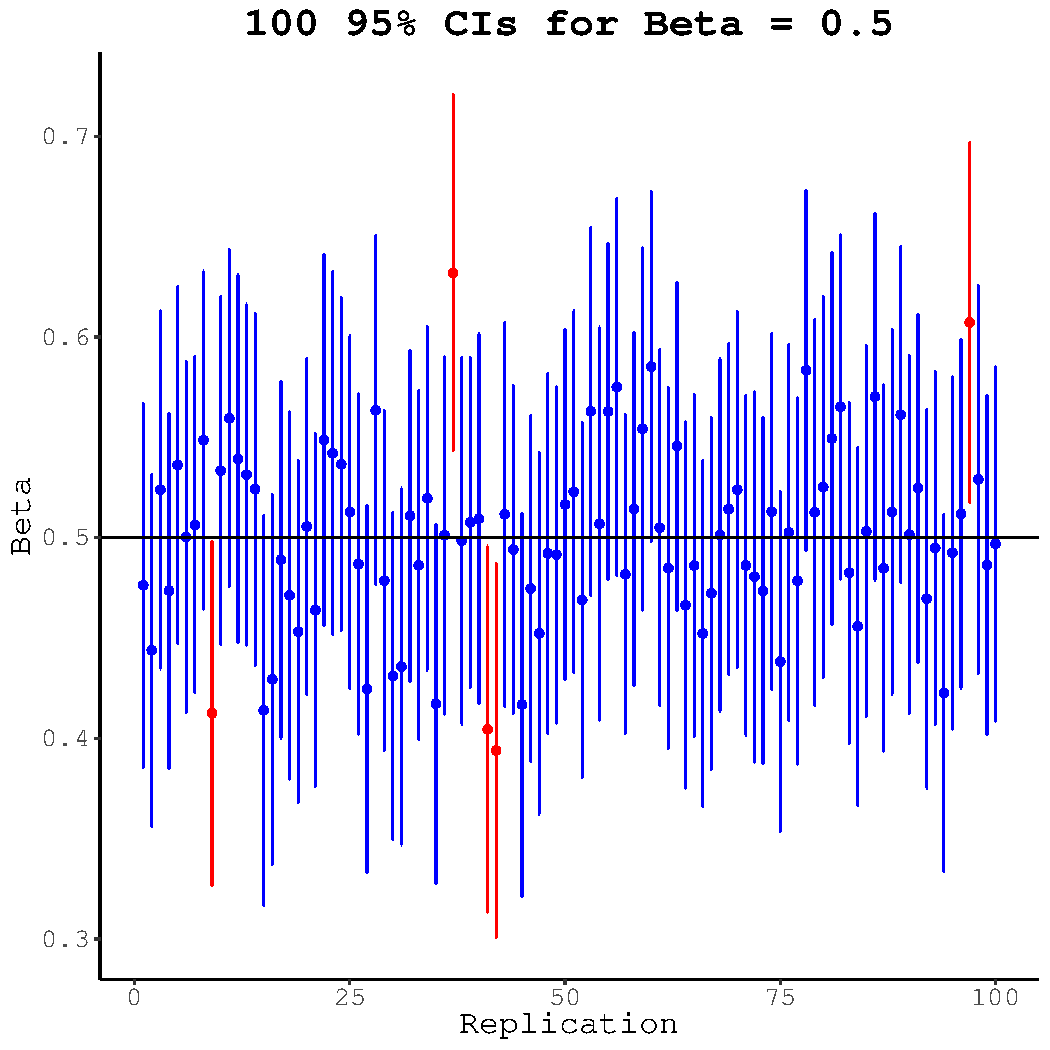
\includegraphics[width=\maxwidth]{figure/unnamed-chunk-21-1} 

}


\end{knitrout}

\end{column}
\end{columns}

\end{frame}

%------------------------------------------------------------------------------%

\begin{frame}{Inference with Confidence Intervals}
  
  CIs give us a plausible range for the population value of $\beta$, so we can 
  use CIs to support inference.
  
\begin{columns}
  \begin{column}{0.5\textwidth}
    
\begin{knitrout}\footnotesize
\definecolor{shadecolor}{rgb}{0.878, 0.918, 0.933}\color{fgcolor}

{\centering 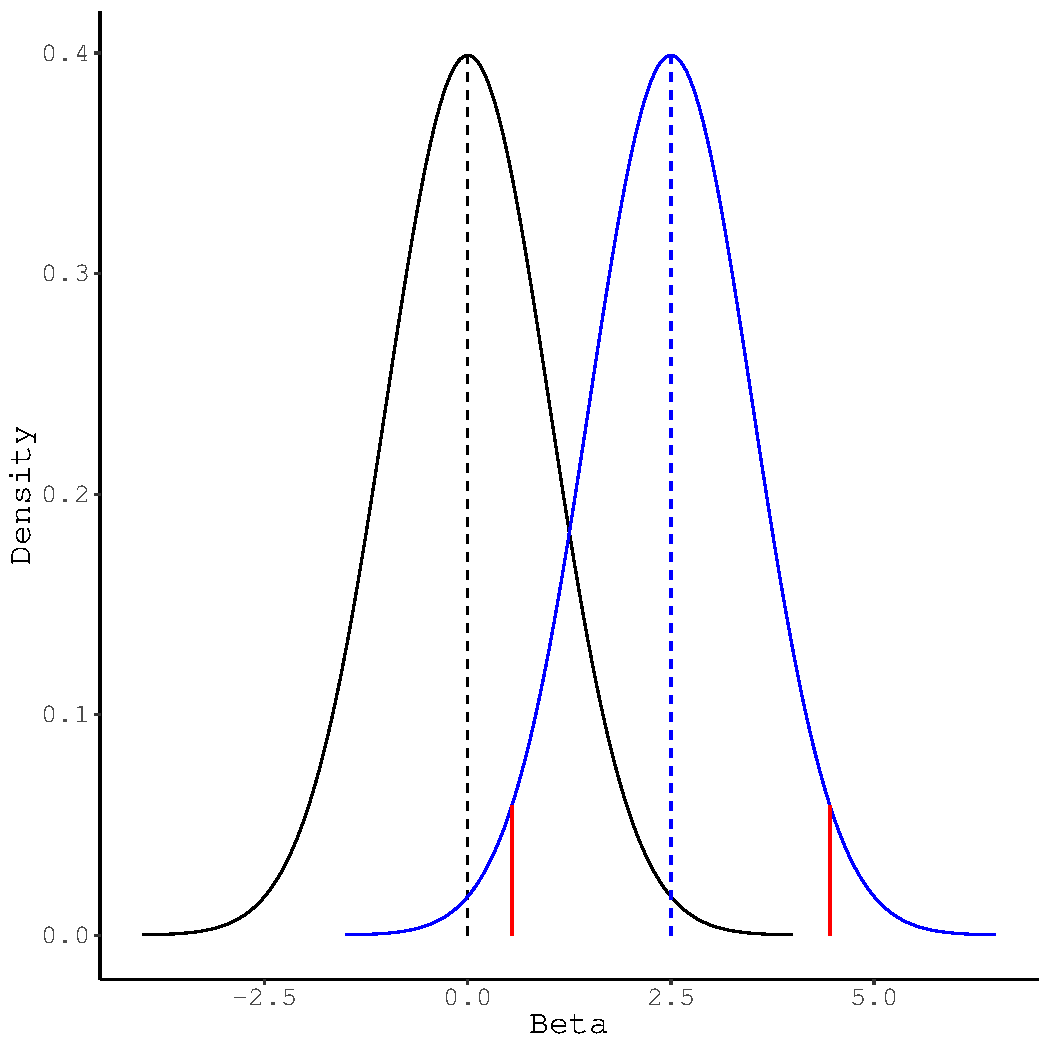
\includegraphics[width=\maxwidth]{figure/unnamed-chunk-22-1} 

}


\end{knitrout}

\end{column}
\begin{column}{0.5\textwidth}
  
\begin{knitrout}\footnotesize
\definecolor{shadecolor}{rgb}{0.878, 0.918, 0.933}\color{fgcolor}

{\centering 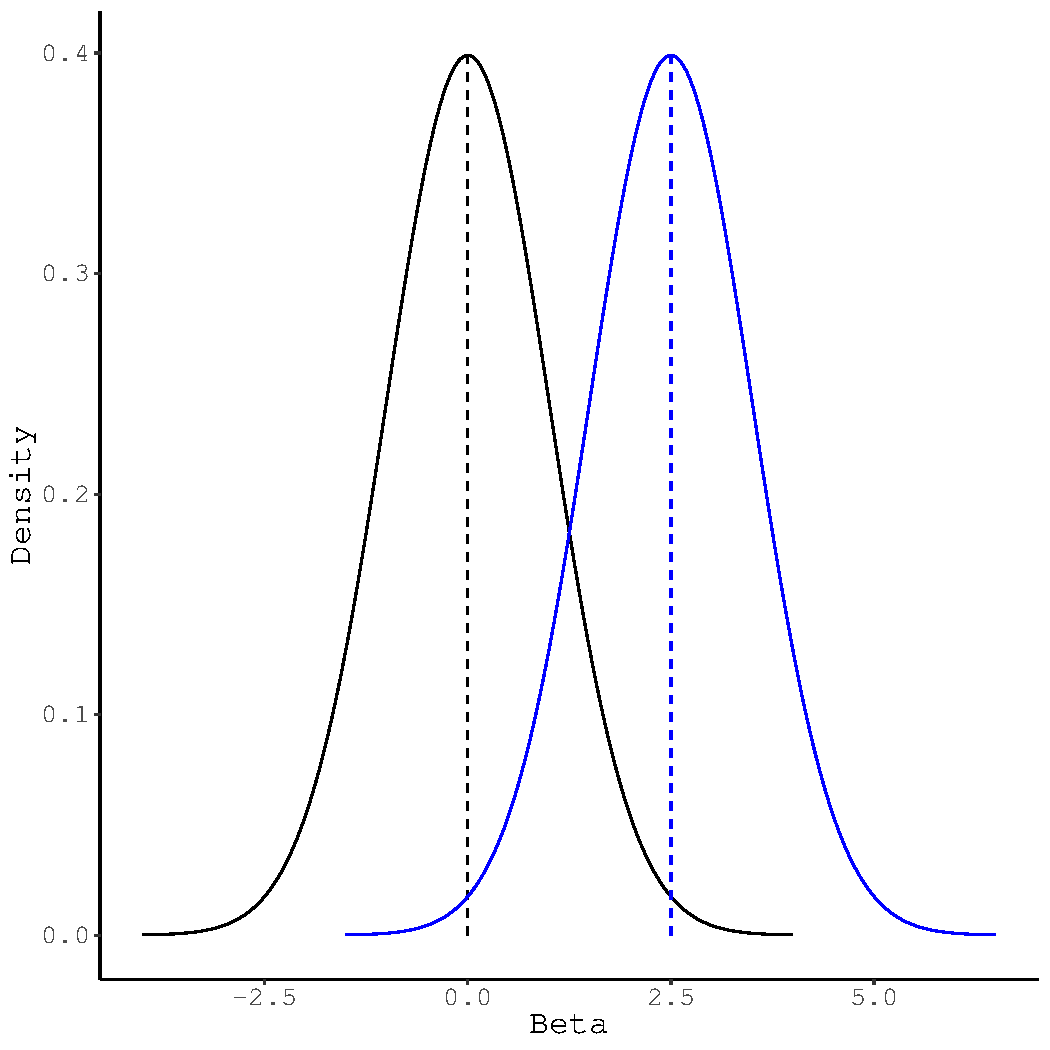
\includegraphics[width=\maxwidth]{figure/unnamed-chunk-23-1} 

}


\end{knitrout}

\end{column}
\end{columns}

\end{frame}
}%%%%%%%%%%%%%%%%%%%%%%%%%%%%%%%%%%%%%%%%%%%%%%%%%%%%%%%%%%%%%%%%%%%%%%%%%%%%%%%

%------------------------------------------------------------------------------%

\begin{frame}{Model-Based Prediction}

  In the social and behavioral sciences, regression modeling is often focused on
  inference about estimated model parameters.
  \vc
  \begin{itemize}
  \item The association between the price of a car and its power.
    \vc
  \item We model the system and scrutinize $\hat{\beta}_1$ to make inferences
    about the association between price and power.
  \end{itemize}
  \vb
  \pause
  In data science applications, we're often more interested in predicting the
  outcome for new observations.
  \vc
  \begin{itemize}
  \item After we estimate $\hat{\beta}_0$ and $\hat{\beta}_1$, we can plug in
    new predictor data and get a predicted outcome value for any new case.
  \vc
  \item In our example, these predictions represent the projected horsepower
    ratings of cars with prices given by the new $X_{price}$ values.
  \end{itemize}

\end{frame}

%------------------------------------------------------------------------------%

\begin{frame}{Inference vs. Prediction}

  When doing statistical inference, we focus on how certain variables relate to
  the outcome.
  \begin{itemize}
  \item Do men have higher job-satisfaction than women?
  \item Does increased spending on advertising correlate with more sales?
  \item Is there a relationship between the number of liquor stores in a
    neighborhood and the amount of crime?
  \end{itemize}

  \vb
  \pause

  When doing prediction (or classification), we want to build a tool that can
  accurately guess future values.
  \begin{itemize}
  \item Will it rain tomorrow?
  \item How much will a company earn from investing in a certain research
    profile?
  \item What is a patients risk of heart disease based on their medical history
    and test results?
  \end{itemize}

\end{frame}

%------------------------------------------------------------------------------%

\sectionslide{Model Fit}

\watermarkoff %----------------------------------------------------------------%

\begin{frame}{Model Fit}
  We may also want to know how well our model explains the outcome.
  \begin{itemize}
  \item Our model explains some proportion of the outcome's variability.
  \item The residual variance $\hat{\sigma}^2 = \text{Var}(\hat{\varepsilon})$
    will be less than $\text{Var}(Y)$.
  \end{itemize}

  \begin{columns}
    \begin{column}{0.4\textwidth}
      \only<1>{
\begin{knitrout}\footnotesize
\definecolor{shadecolor}{rgb}{0.878, 0.918, 0.933}\color{fgcolor}

{\centering 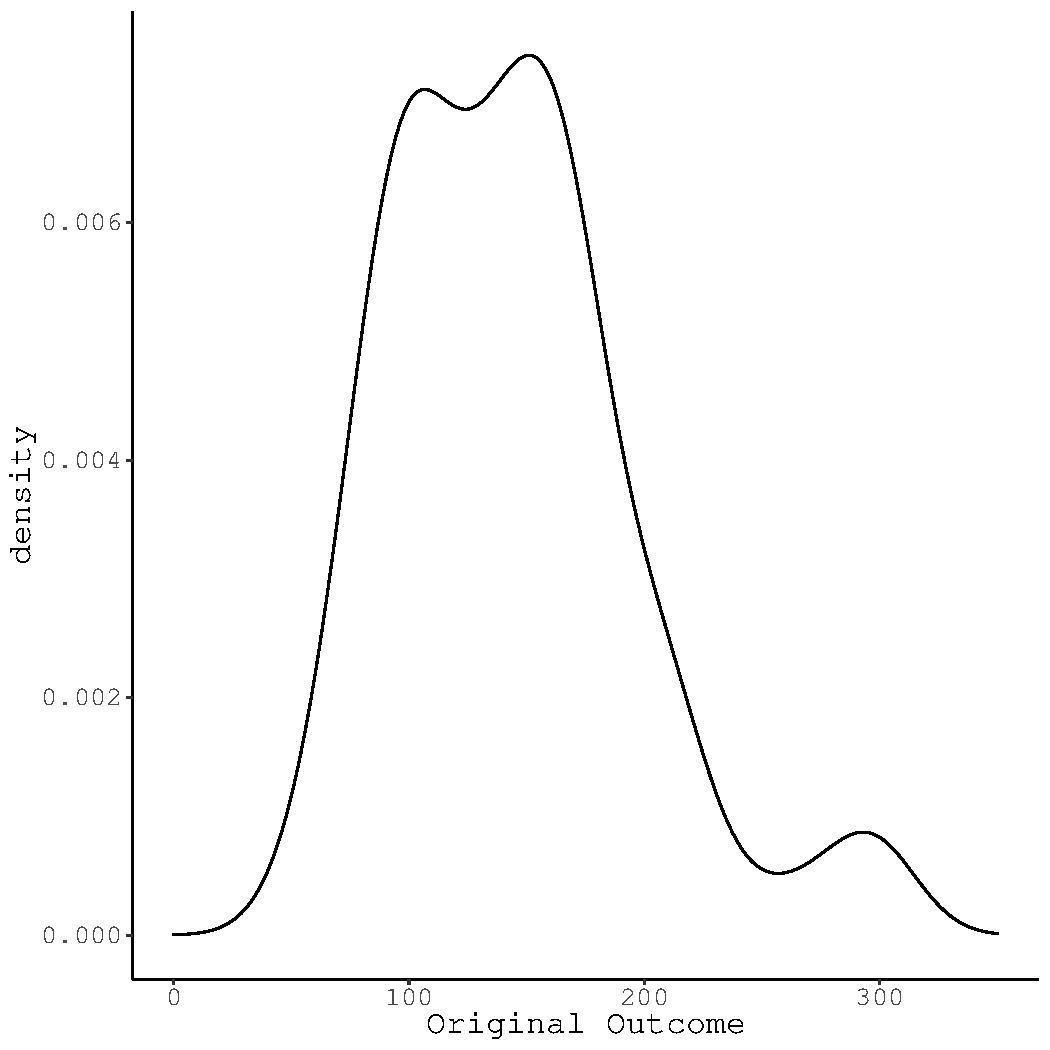
\includegraphics[width=\maxwidth]{figure/unnamed-chunk-24-1} 

}


\end{knitrout}
      }
      \only<2>{
\begin{knitrout}\footnotesize
\definecolor{shadecolor}{rgb}{0.878, 0.918, 0.933}\color{fgcolor}

{\centering 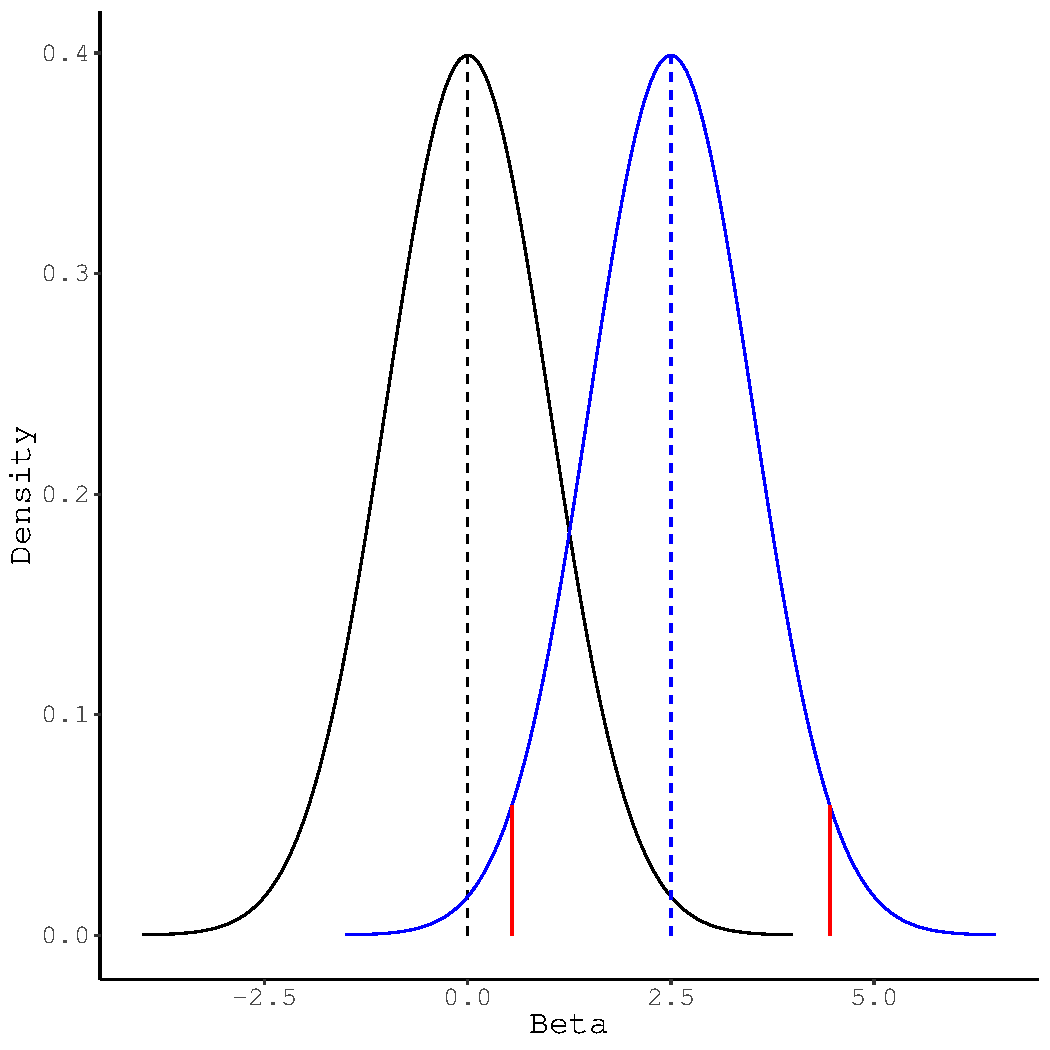
\includegraphics[width=\maxwidth]{figure/unnamed-chunk-25-1} 

}


\end{knitrout}
      }
    \end{column}
    \begin{column}{0.1\textwidth}

      \Huge{$\rightarrow$}

    \end{column}
    \begin{column}{0.4\textwidth}

      \only<1>{
\begin{knitrout}\footnotesize
\definecolor{shadecolor}{rgb}{0.878, 0.918, 0.933}\color{fgcolor}

{\centering 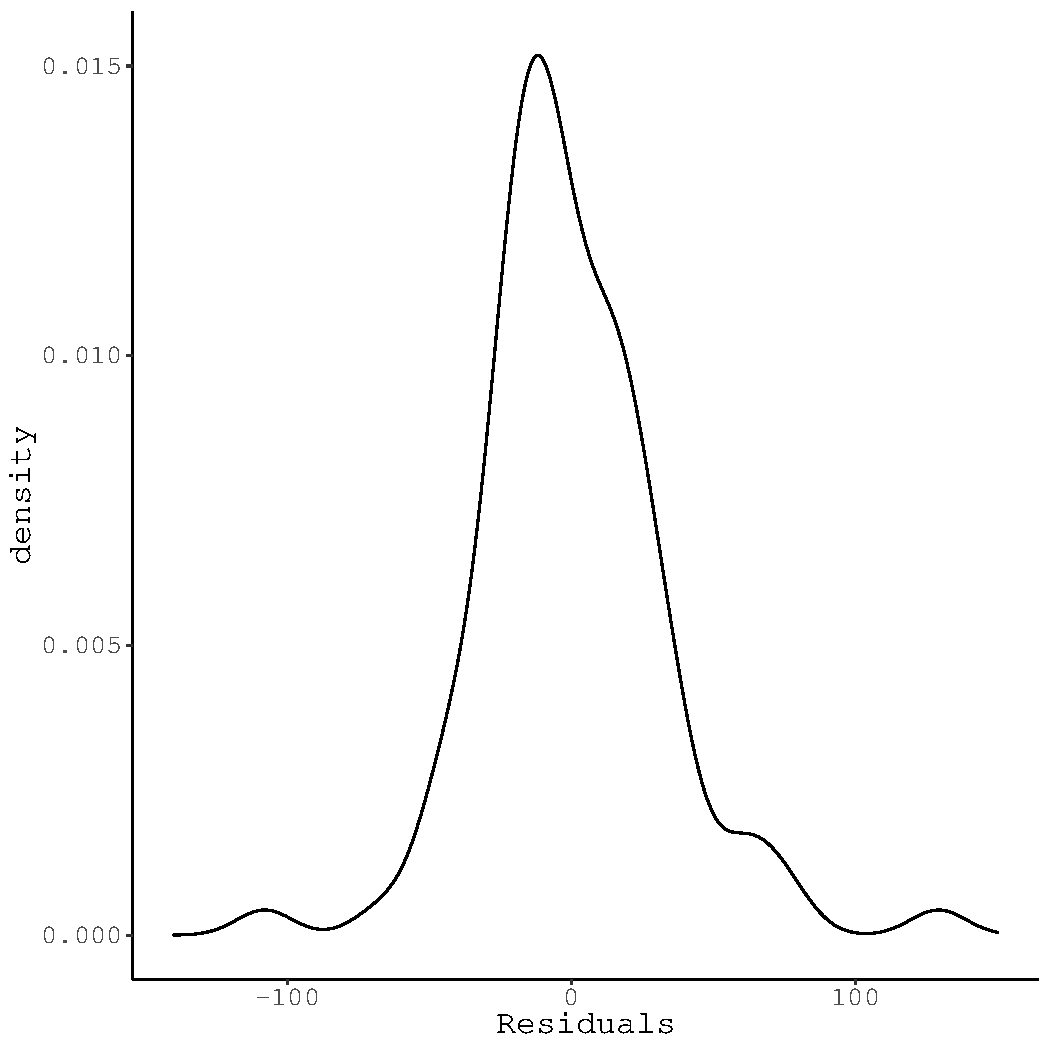
\includegraphics[width=\maxwidth]{figure/unnamed-chunk-26-1} 

}


\end{knitrout}
      }
      \only<2>{

\begin{knitrout}\footnotesize
\definecolor{shadecolor}{rgb}{0.878, 0.918, 0.933}\color{fgcolor}

{\centering 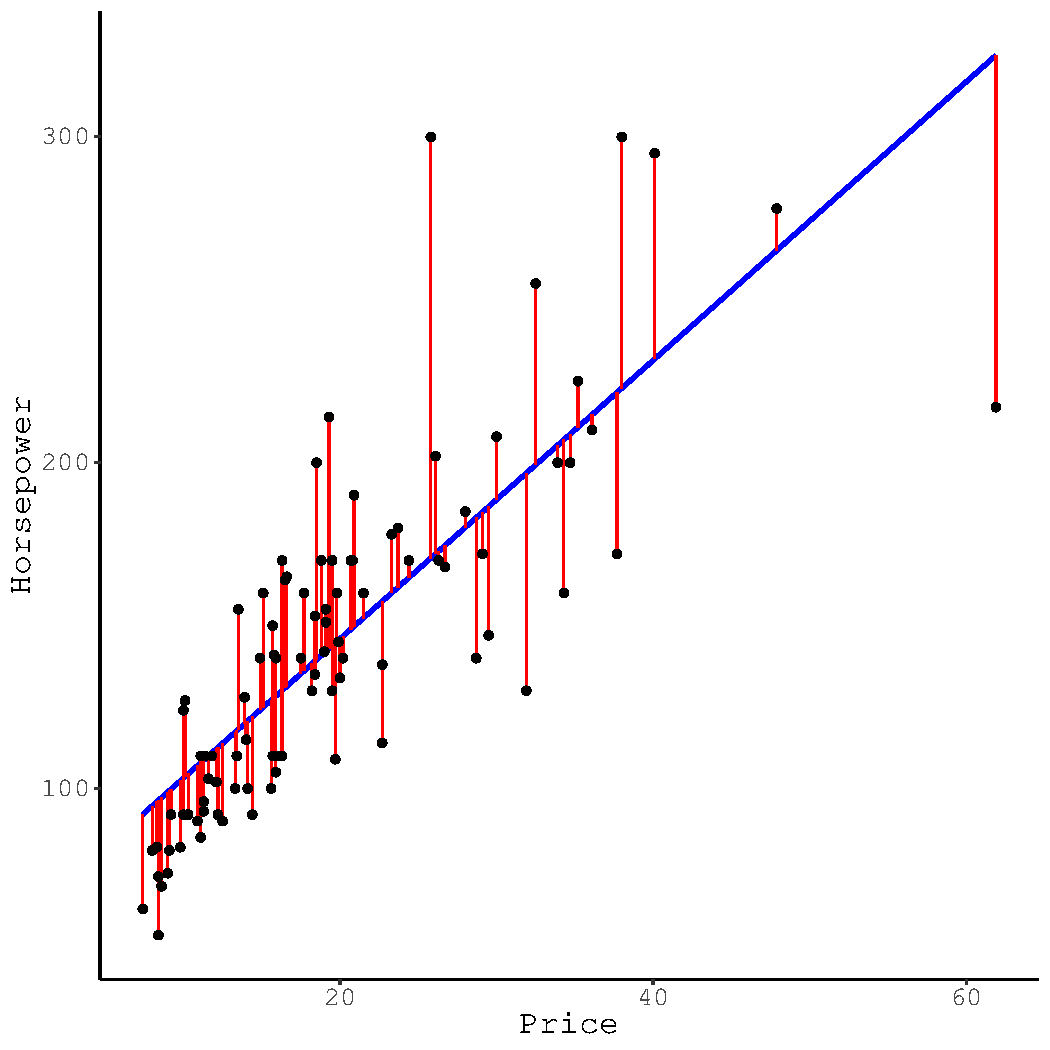
\includegraphics[width=\maxwidth]{figure/unnamed-chunk-27-1} 

}


\end{knitrout}
      }

    \end{column}
  \end{columns}

\end{frame}

\watermarkon %-----------------------------------------------------------------%

\begin{frame}[shrink = 5]{Model Fit}

  We quantify the proportion of the outcome's variance that is explained by our
  model using the $R^2$ statistic:
  \begin{align*}
    R^2 = \frac{TSS - RSS}{TSS} = 1 - \frac{RSS}{TSS}
  \end{align*}
  where
  \begin{align*}
    TSS = \sum_{n = 1}^N \left(Y_n - \bar{Y}\right)^2 =
    \text{Var}(Y)\times (N - 1)
  \end{align*}



For our example problem, we get:
\begin{align*}
  R^2 = 1 - \frac{95573}{252363} \approx
  0.62
\end{align*}
Indicating that car price explains 62\% of the variability in
horsepower.

\end{frame}

%------------------------------------------------------------------------------%

\begin{frame}{Model Fit for Prediction}

  When assessing predictive performance, we will most often use the \emph{mean
    squared error} (MSE) as our criterion.
  \vb
  \begin{align*}
    MSE &= \frac{1}{N} \sum_{n = 1}^N \left(Y_n - \hat{Y}_n\right)^2\\
    &= \frac{1}{N} \sum_{n = 1}^N \left(Y_n - \hat{\beta}_0 -
    \sum_{p = 1}^P \hat{\beta}_p X_{np} \right)^2\\
    &= \frac{RSS}{N}
  \end{align*}



For our example problem, we get:
\begin{align*}
  MSE = \frac{95573}{93} \approx 1027.67
\end{align*}

\end{frame}

%------------------------------------------------------------------------------%

\begin{frame}{Interpreting MSE}



  The MSE quantifies the average squared prediction error.
  \begin{itemize}
  \item Taking the square root improves interpretation.
  \end{itemize}
  \begin{align*}
    RMSE = \sqrt{MSE}
  \end{align*}
  The RMSE estimates the magnitude of the expected prediction error.
  \begin{itemize}
  \item For our example problem, we get:
  \end{itemize}
  \begin{align*}
    RMSE = \sqrt{\frac{95573}{93}} \approx
    32.06
  \end{align*}
  \vx{-8}
  \begin{itemize}
  \item When using price as the only predictor of horsepower, we expect
    prediction errors with magnitudes of 32.06 horsepower.
  \end{itemize}

\end{frame}

%------------------------------------------------------------------------------%

\begin{frame}{AIC}

\end{frame}

%------------------------------------------------------------------------------%

\sectionslide{Multiple Linear Regression}

\watermarkoff %----------------------------------------------------------------%

\begin{frame}{Graphical Representations of Regression Models}

  A regression of two variables can be represented on a 2D scatterplot.
  \begin{itemize}
  \item Simple linear regression implies a 1D line in 2D space.
  \end{itemize}
  \vb
  \begin{columns}
    \begin{column}{0.45\textwidth}

\begin{knitrout}\footnotesize
\definecolor{shadecolor}{rgb}{0.878, 0.918, 0.933}\color{fgcolor}

{\centering 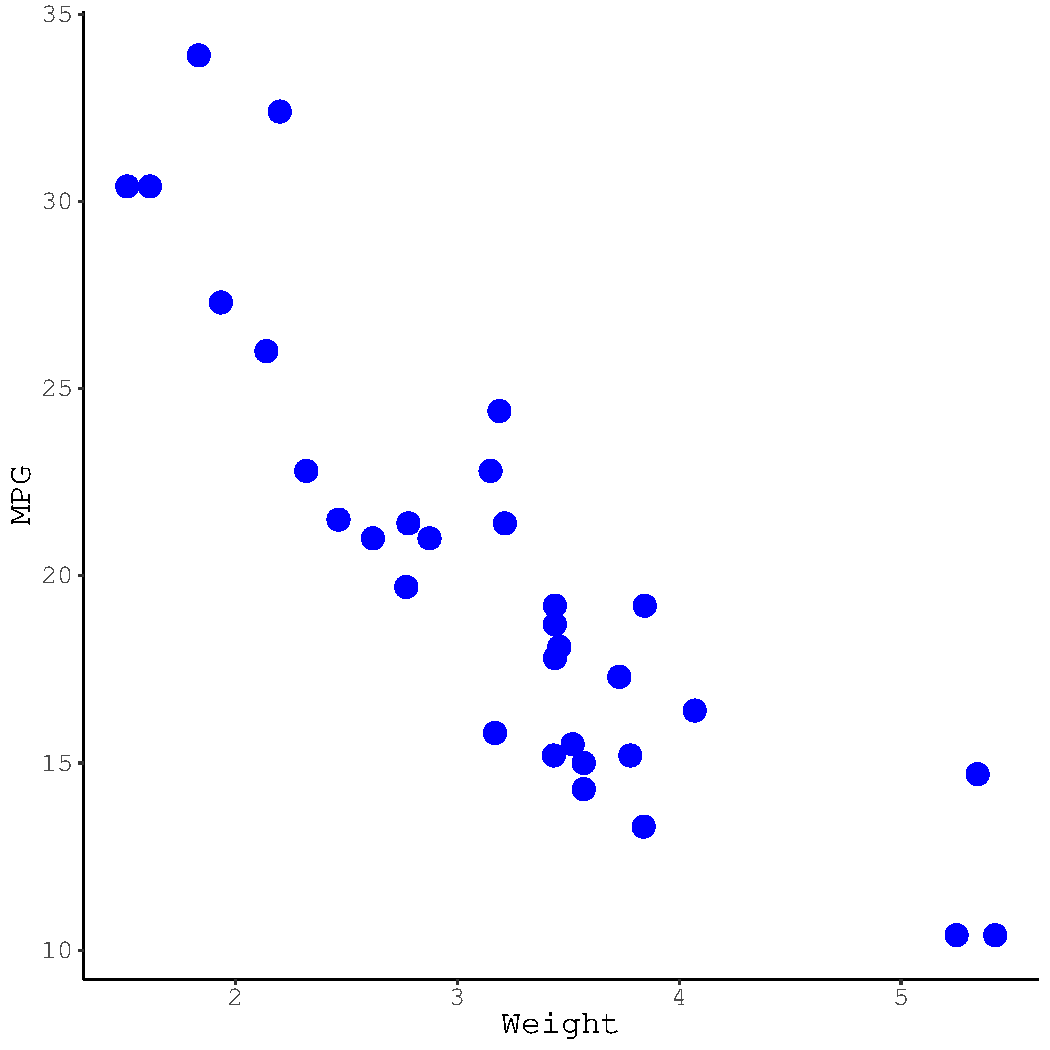
\includegraphics[width=\maxwidth]{figure/unnamed-chunk-31-1} 

}


\end{knitrout}

\end{column}

\begin{column}{0.1\textwidth}

  \begin{center}\huge{$\rightarrow$}\end{center}

\end{column}

\begin{column}{0.45\textwidth}

\begin{knitrout}\footnotesize
\definecolor{shadecolor}{rgb}{0.878, 0.918, 0.933}\color{fgcolor}

{\centering 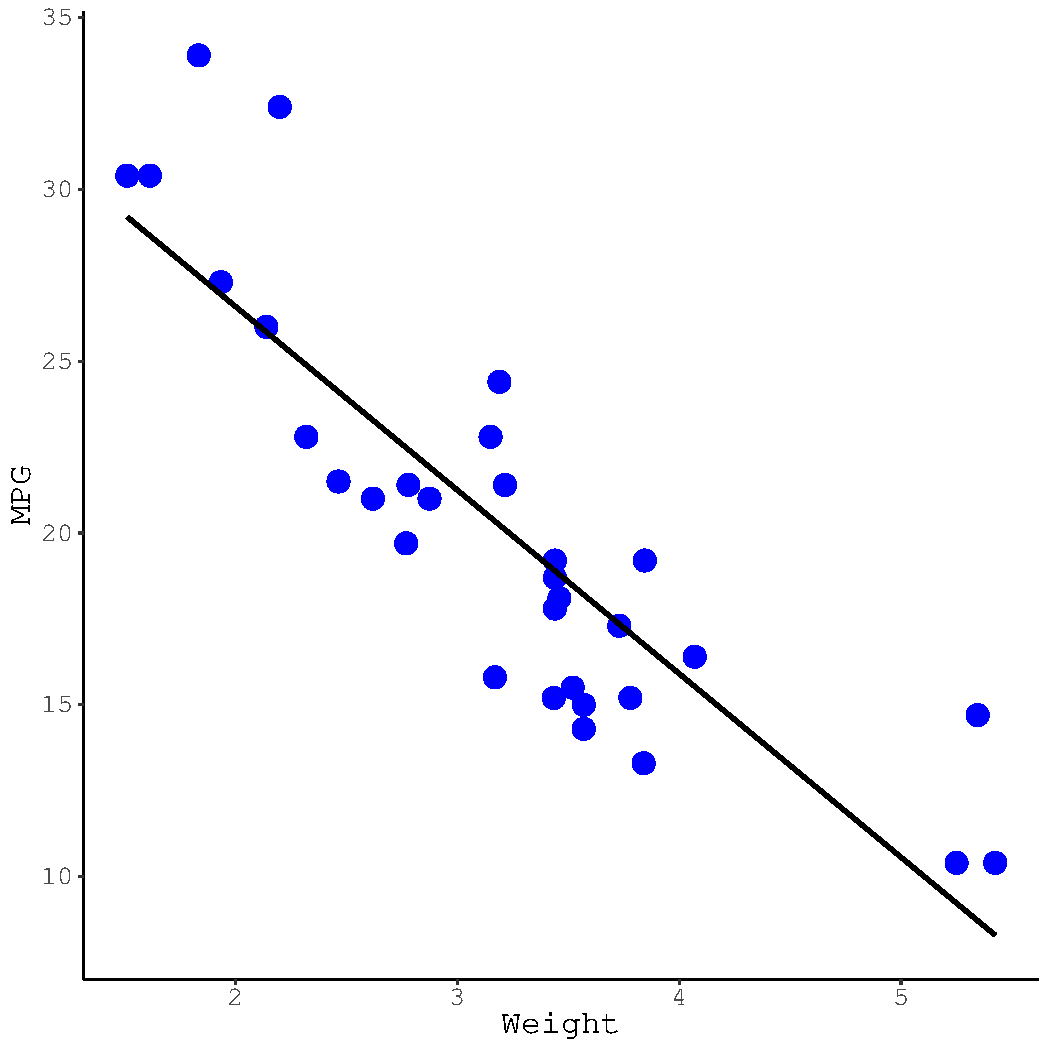
\includegraphics[width=\maxwidth]{figure/unnamed-chunk-32-1} 

}


\end{knitrout}

\end{column}
\end{columns}

\end{frame}

%------------------------------------------------------------------------------%

\begin{frame}{Graphical Representations of Regression Models}

  Adding an additional predictor leads to a 3D point cloud.
  \vb
  \begin{itemize}
  \item A regression model with two IVs implies a 2D plane in 3D space.
  \end{itemize}

  \begin{columns}
    \begin{column}{0.45\textwidth}

      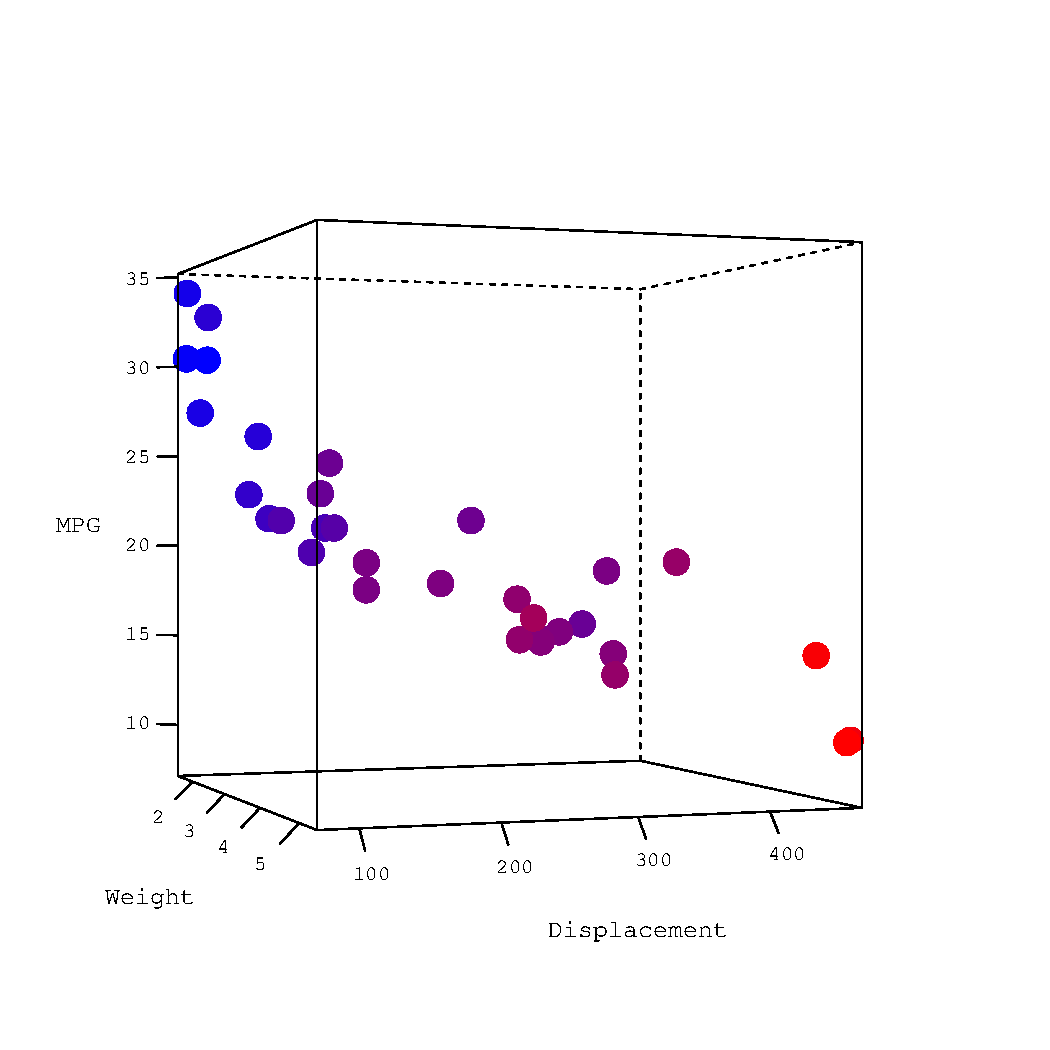
\includegraphics[width = 1.2\textwidth]{figures/3d_data_plot}

    \end{column}

    \begin{column}{0.1\textwidth}

      \begin{center}\huge{$~~~~\rightarrow$}\end{center}

    \end{column}

    \begin{column}{0.45\textwidth}

      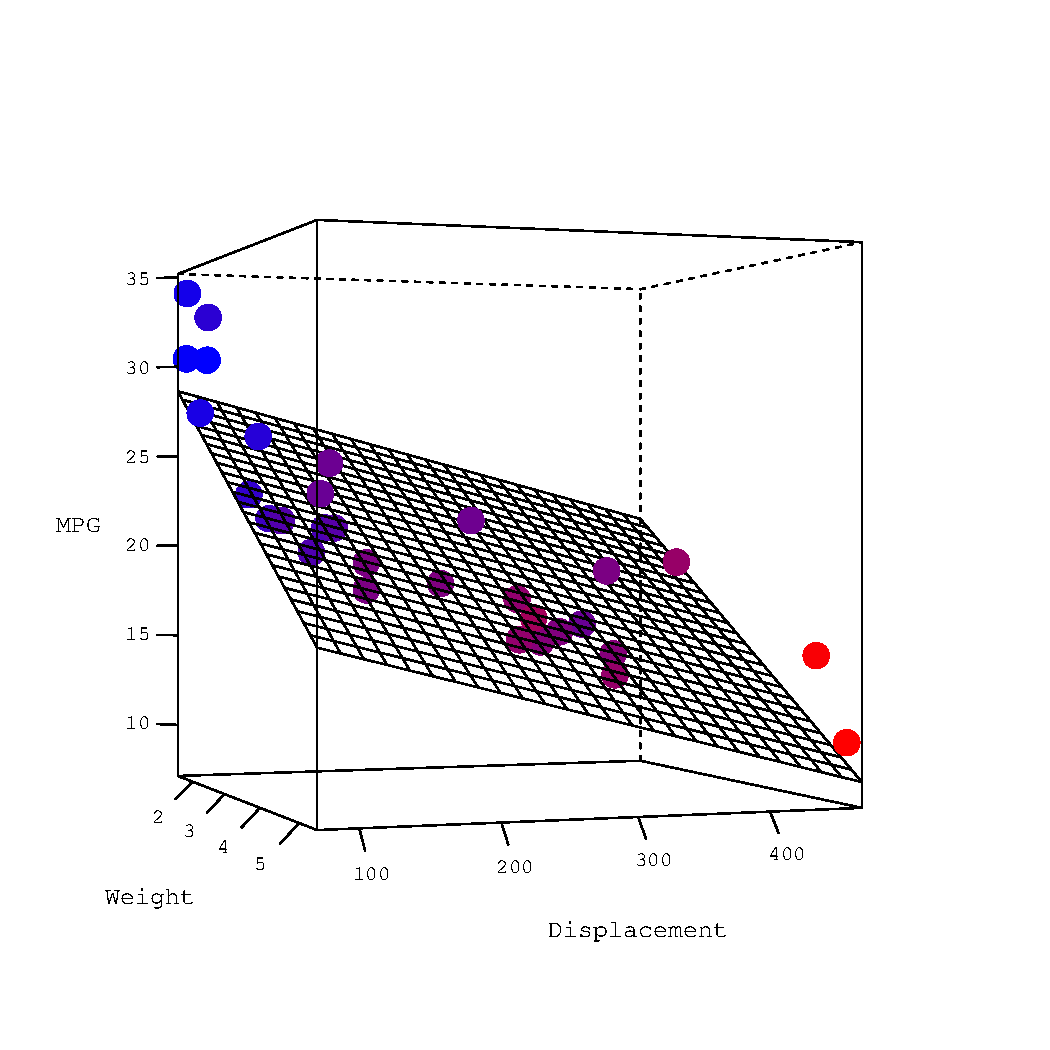
\includegraphics[width = 1.2\textwidth]{figures/response_surface_plot}

    \end{column}
  \end{columns}

\end{frame}

\watermarkon %-----------------------------------------------------------------%

\begin{frame}{Partial Effects}

  In MLR, we want to examine the \emph{partial effects} of the predictors.
  \vb
  \begin{itemize}
  \item What is the effect of a predictor after controlling for some other set
    of variables?
  \end{itemize}
  \va
  This approach is crucial to controlling confounds and adequately modeling
  real-world phenomena.

\end{frame}

%------------------------------------------------------------------------------%

\begin{frame}[fragile]{Example}

\begin{knitrout}\footnotesize
\definecolor{shadecolor}{rgb}{0.878, 0.918, 0.933}\color{fgcolor}\begin{kframe}
\begin{alltt}
\hlcom{## Read in the 'diabetes' dataset:}
\hlstd{dDat} \hlkwb{<-} \hlkwd{readRDS}\hlstd{(}\hlstr{"../data/diabetes.rds"}\hlstd{)}

\hlcom{## Simple regression with which we're familiar:}
\hlstd{out1} \hlkwb{<-} \hlkwd{lm}\hlstd{(bp} \hlopt{~} \hlstd{age,} \hlkwc{data} \hlstd{= dDat)}
\end{alltt}
\end{kframe}
\end{knitrout}

\va

\textsc{Asking}: What is the effect of age on average blood pressure?

\end{frame}

\watermarkoff %----------------------------------------------------------------%

\begin{frame}[allowframebreaks, fragile]{Example}

\begin{knitrout}\footnotesize
\definecolor{shadecolor}{rgb}{0.878, 0.918, 0.933}\color{fgcolor}\begin{kframe}
\begin{alltt}
\hlkwd{partSummary}\hlstd{(out1,} \hlopt{-}\hlnum{1}\hlstd{)}
\end{alltt}
\begin{verbatim}
## Residuals:
##     Min      1Q  Median      3Q     Max 
## -31.188  -8.897  -1.209   8.612  39.952 
## 
## Coefficients:
##             Estimate Std. Error t value Pr(>|t|)
## (Intercept) 77.47605    2.38132  32.535  < 2e-16
## age          0.35391    0.04739   7.469 4.39e-13
## 
## Residual standard error: 13.04 on 440 degrees of freedom
## Multiple R-squared:  0.1125,	Adjusted R-squared:  0.1105 
## F-statistic: 55.78 on 1 and 440 DF,  p-value: 4.393e-13
\end{verbatim}
\end{kframe}
\end{knitrout}

\end{frame}

\watermarkon %-----------------------------------------------------------------%

\begin{frame}[fragile]{Example}

\begin{knitrout}\footnotesize
\definecolor{shadecolor}{rgb}{0.878, 0.918, 0.933}\color{fgcolor}\begin{kframe}
\begin{alltt}
\hlcom{## Add in another predictor:}
\hlstd{out2} \hlkwb{<-} \hlkwd{lm}\hlstd{(bp} \hlopt{~} \hlstd{age} \hlopt{+} \hlstd{bmi,} \hlkwc{data} \hlstd{= dDat)}
\end{alltt}
\end{kframe}
\end{knitrout}

\va

\textsc{Asking}: What is the effect of BMI on average blood pressure,
\emph{after controlling for age?}
\vb
\begin{itemize}
  \item We're partialing age out of the effect of BMI on blood pressure.
\end{itemize}

\end{frame}

\watermarkoff %----------------------------------------------------------------%

\begin{frame}[allowframebreaks, fragile]{Example}

\begin{knitrout}\footnotesize
\definecolor{shadecolor}{rgb}{0.878, 0.918, 0.933}\color{fgcolor}\begin{kframe}
\begin{alltt}
\hlkwd{partSummary}\hlstd{(out2,} \hlopt{-}\hlnum{1}\hlstd{)}
\end{alltt}
\begin{verbatim}
## Residuals:
##     Min      1Q  Median      3Q     Max 
## -29.287  -8.198  -0.178   8.413  41.026 
## 
## Coefficients:
##             Estimate Std. Error t value Pr(>|t|)
## (Intercept) 52.24654    3.83168  13.635  < 2e-16
## age          0.28651    0.04504   6.362 5.02e-10
## bmi          1.08053    0.13363   8.086 6.06e-15
## 
## Residual standard error: 12.18 on 439 degrees of freedom
## Multiple R-squared:  0.2276,	Adjusted R-squared:  0.224 
## F-statistic: 64.66 on 2 and 439 DF,  p-value: < 2.2e-16
\end{verbatim}
\end{kframe}
\end{knitrout}

\end{frame}

%------------------------------------------------------------------------------%

\begin{frame}[fragile]{Interpretation}

  \begin{columns}
    \begin{column}{0.5\textwidth}

      \begin{itemize}
      \item The expected average blood pressure for an unborn patient with a
        negligible extent is 52.25.
        \vb
      \item For each year older, average blood pressure is expected to increase
        by 0.29 points, after controlling for
        BMI.
        \vb
      \item For each additional point of BMI, average blood pressure is
        expected to increase by 1.08 points,
        after controlling for age.
      \end{itemize}

    \end{column}

    \begin{column}{0.5\textwidth}

      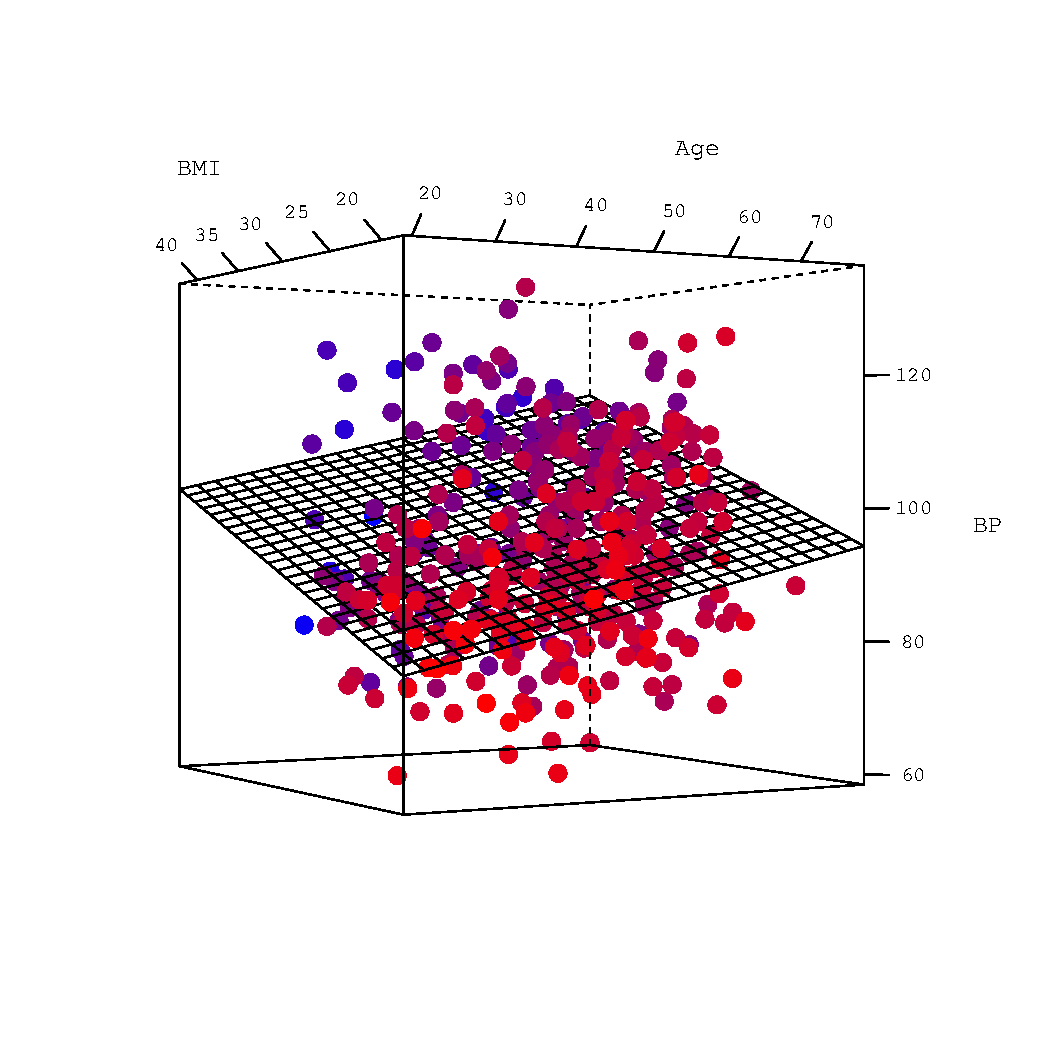
\includegraphics[width = 1.1\textwidth]{figures/response_surface_plot2}

    \end{column}
  \end{columns}

\end{frame}

%------------------------------------------------------------------------------%

\begin{frame}[fragile]{Multiple $R^2$}

  How much variation in blood pressure is explained by the two models?
  \begin{itemize}
    \item Check the $R^2$ values.
  \end{itemize}

\begin{knitrout}\footnotesize
\definecolor{shadecolor}{rgb}{0.878, 0.918, 0.933}\color{fgcolor}\begin{kframe}
\begin{alltt}
\hlcom{## Extract R^2 values:}
\hlstd{r2.1} \hlkwb{<-} \hlkwd{summary}\hlstd{(out1)}\hlopt{$}\hlstd{r.squared}
\hlstd{r2.2} \hlkwb{<-} \hlkwd{summary}\hlstd{(out2)}\hlopt{$}\hlstd{r.squared}

\hlstd{r2.1}
\end{alltt}
\begin{verbatim}
## [1] 0.1125117
\end{verbatim}
\begin{alltt}
\hlstd{r2.2}
\end{alltt}
\begin{verbatim}
## [1] 0.2275606
\end{verbatim}
\end{kframe}
\end{knitrout}

\end{frame}

%------------------------------------------------------------------------------%

\begin{frame}[fragile, allowframebreaks]{F-Statistic}

  How do we know if the $R^2$ values are significantly greater than zero?
  \begin{itemize}
  \item We use the F-statistic to test $H_0: R^2 = 0$ vs. $H_1: R^2 > 0$.
  \end{itemize}

\begin{knitrout}\footnotesize
\definecolor{shadecolor}{rgb}{0.878, 0.918, 0.933}\color{fgcolor}\begin{kframe}
\begin{alltt}
\hlstd{f1} \hlkwb{<-} \hlkwd{summary}\hlstd{(out1)}\hlopt{$}\hlstd{fstatistic}
\hlstd{f1}
\end{alltt}
\begin{verbatim}
##     value     numdf     dendf 
##  55.78116   1.00000 440.00000
\end{verbatim}
\begin{alltt}
\hlkwd{pf}\hlstd{(}\hlkwc{q} \hlstd{= f1[}\hlnum{1}\hlstd{],} \hlkwc{df1} \hlstd{= f1[}\hlnum{2}\hlstd{],} \hlkwc{df2} \hlstd{= f1[}\hlnum{3}\hlstd{],} \hlkwc{lower.tail} \hlstd{=} \hlnum{FALSE}\hlstd{)}
\end{alltt}
\begin{verbatim}
##        value 
## 4.392569e-13
\end{verbatim}
\end{kframe}
\end{knitrout}

\pagebreak

\begin{knitrout}\footnotesize
\definecolor{shadecolor}{rgb}{0.878, 0.918, 0.933}\color{fgcolor}\begin{kframe}
\begin{alltt}
\hlstd{f2} \hlkwb{<-} \hlkwd{summary}\hlstd{(out2)}\hlopt{$}\hlstd{fstatistic}
\hlstd{f2}
\end{alltt}
\begin{verbatim}
##    value    numdf    dendf 
##  64.6647   2.0000 439.0000
\end{verbatim}
\begin{alltt}
\hlkwd{pf}\hlstd{(f2[}\hlnum{1}\hlstd{], f2[}\hlnum{2}\hlstd{], f2[}\hlnum{3}\hlstd{],} \hlkwc{lower.tail} \hlstd{=} \hlnum{FALSE}\hlstd{)}
\end{alltt}
\begin{verbatim}
##        value 
## 2.433518e-25
\end{verbatim}
\end{kframe}
\end{knitrout}

\end{frame}

%------------------------------------------------------------------------------%

\begin{frame}[fragile]{Comparing Models}

  How do we quantify the additional variation explained by BMI, above and beyond
  age?
  \begin{itemize}
  \item Compute the $\Delta R^2$
  \end{itemize}

\begin{knitrout}\footnotesize
\definecolor{shadecolor}{rgb}{0.878, 0.918, 0.933}\color{fgcolor}\begin{kframe}
\begin{alltt}
\hlcom{## Compute change in R^2:}
\hlstd{r2.2} \hlopt{-} \hlstd{r2.1}
\end{alltt}
\begin{verbatim}
## [1] 0.115049
\end{verbatim}
\end{kframe}
\end{knitrout}

\end{frame}

%------------------------------------------------------------------------------%

\begin{frame}[fragile]{Significance Testing}

How do we know if $\Delta R^2$ represents a significantly greater degree of
explained variation?
\begin{itemize}
\item Use an $F$-test for $H_0: \Delta R^2 = 0$ vs. $H_1: \Delta R^2 > 0$
\end{itemize}

\begin{knitrout}\footnotesize
\definecolor{shadecolor}{rgb}{0.878, 0.918, 0.933}\color{fgcolor}\begin{kframe}
\begin{alltt}
\hlcom{## Is that increase significantly greater than zero?}
\hlkwd{anova}\hlstd{(out1, out2)}
\end{alltt}
\begin{verbatim}
## Analysis of Variance Table
## 
## Model 1: bp ~ age
## Model 2: bp ~ age + bmi
##   Res.Df   RSS Df Sum of Sq      F    Pr(>F)    
## 1    440 74873                                  
## 2    439 65167  1    9706.1 65.386 6.057e-15 ***
## ---
## Signif. codes:  
## 0 '***' 0.001 '**' 0.01 '*' 0.05 '.' 0.1 ' ' 1
\end{verbatim}
\end{kframe}
\end{knitrout}

\end{frame}

%------------------------------------------------------------------------------%

\begin{frame}[fragile]{Model Comparison}

  We can also compare models based on their prediction errors.
  \begin{itemize}
  \item For OLS regression, we usually compare MSE values.
  \end{itemize}
  \vx{-6}
\begin{knitrout}\footnotesize
\definecolor{shadecolor}{rgb}{0.878, 0.918, 0.933}\color{fgcolor}\begin{kframe}
\begin{alltt}
\hlstd{mse1} \hlkwb{<-} \hlkwd{MSE}\hlstd{(}\hlkwc{y_pred} \hlstd{=} \hlkwd{predict}\hlstd{(out1),} \hlkwc{y_true} \hlstd{= dDat}\hlopt{$}\hlstd{bp)}
\hlstd{mse2} \hlkwb{<-} \hlkwd{MSE}\hlstd{(}\hlkwc{y_pred} \hlstd{=} \hlkwd{predict}\hlstd{(out2),} \hlkwc{y_true} \hlstd{= dDat}\hlopt{$}\hlstd{bp)}

\hlstd{mse1}
\end{alltt}
\begin{verbatim}
## [1] 169.3963
\end{verbatim}
\begin{alltt}
\hlstd{mse2}
\end{alltt}
\begin{verbatim}
## [1] 147.4367
\end{verbatim}
\end{kframe}
\end{knitrout}

In this case, the MSE for the model with $BMI$ included is smaller.
\begin{itemize}
\item We should prefer the the larger model.
\end{itemize}

\end{frame}

\end{document}

%------------------------------------------------------------------------------%
%------------------------------------------------------------------------------%
%------------------------------------------------------------------------------%
%------------------------------------------------------------------------------%
%------------------------------------------------------------------------------%
%------------------------------------------------------------------------------%
%------------------------------------------------------------------------------%
%------------------------------------------------------------------------------%
%------------------------------------------------------------------------------%
%------------------------------------------------------------------------------%

\begin{frame}[fragile]{Model-Building Example}

  Let's walk through an example of the model-building process.
  \vc
  \begin{itemize}
    \item We'll take $Y_{bp} = \beta_0 + \beta_1 X_{age.30} + \varepsilon$ as
      our baseline model.
      \vc
    \item Next, we simultaneously add predictors of LDL and HDL cholesterol.
  \end{itemize}
\begin{knitrout}\footnotesize
\definecolor{shadecolor}{rgb}{0.878, 0.918, 0.933}\color{fgcolor}\begin{kframe}
\begin{alltt}
\hlcom{## Center predictor variables:}
\hlstd{dDat}\hlopt{$}\hlstd{ldl100} \hlkwb{<-} \hlstd{dDat}\hlopt{$}\hlstd{ldl} \hlopt{-} \hlnum{100}
\hlstd{dDat}\hlopt{$}\hlstd{hdl60}  \hlkwb{<-} \hlstd{dDat}\hlopt{$}\hlstd{hdl} \hlopt{-} \hlnum{60}
\hlstd{dDat}\hlopt{$}\hlstd{age30}  \hlkwb{<-} \hlstd{dDat}\hlopt{$}\hlstd{age} \hlopt{-} \hlnum{30}

\hlcom{## Baseline model:}
\hlstd{out1} \hlkwb{<-} \hlkwd{lm}\hlstd{(bp} \hlopt{~} \hlstd{age30,} \hlkwc{data} \hlstd{= dDat)}

\hlcom{## Simultaneously add two predictors:}
\hlstd{out2} \hlkwb{<-} \hlkwd{lm}\hlstd{(bp} \hlopt{~} \hlstd{age30} \hlopt{+} \hlstd{ldl100} \hlopt{+} \hlstd{hdl60,} \hlkwc{data} \hlstd{= dDat)}
\end{alltt}
\end{kframe}
\end{knitrout}

\end{frame}

%------------------------------------------------------------------------------%

\begin{frame}[allowframebreaks, fragile]{Model-Building Example}

\begin{knitrout}\footnotesize
\definecolor{shadecolor}{rgb}{0.878, 0.918, 0.933}\color{fgcolor}\begin{kframe}
\begin{alltt}
\hlkwd{partSummary}\hlstd{(out1,} \hlopt{-}\hlnum{1}\hlstd{)}
\end{alltt}
\begin{verbatim}
## Residuals:
##     Min      1Q  Median      3Q     Max 
## -31.188  -8.897  -1.209   8.612  39.952 
## 
## Coefficients:
##             Estimate Std. Error t value Pr(>|t|)
## (Intercept) 88.09330    1.07470  81.970  < 2e-16
## age30        0.35391    0.04739   7.469 4.39e-13
## 
## Residual standard error: 13.04 on 440 degrees of freedom
## Multiple R-squared:  0.1125,	Adjusted R-squared:  0.1105 
## F-statistic: 55.78 on 1 and 440 DF,  p-value: 4.393e-13
\end{verbatim}
\end{kframe}
\end{knitrout}

\pagebreak

\begin{knitrout}\footnotesize
\definecolor{shadecolor}{rgb}{0.878, 0.918, 0.933}\color{fgcolor}\begin{kframe}
\begin{alltt}
\hlkwd{partSummary}\hlstd{(out2,} \hlopt{-}\hlnum{1}\hlstd{)}
\end{alltt}
\begin{verbatim}
## Residuals:
##     Min      1Q  Median      3Q     Max 
## -33.297  -8.106  -0.979   8.141  40.677 
## 
## Coefficients:
##             Estimate Std. Error t value Pr(>|t|)
## (Intercept) 86.53984    1.13885  75.989  < 2e-16
## age30        0.32178    0.04784   6.727 5.43e-11
## ldl100       0.04166    0.02097   1.987  0.04757
## hdl60       -0.14740    0.04824  -3.055  0.00239
## 
## Residual standard error: 12.84 on 438 degrees of freedom
## Multiple R-squared:  0.1439,	Adjusted R-squared:  0.1381 
## F-statistic: 24.55 on 3 and 438 DF,  p-value: 1.064e-14
\end{verbatim}
\end{kframe}
\end{knitrout}

\end{frame}

\watermarkon %-----------------------------------------------------------------%

\begin{frame}{Interpretations}

  \begin{itemize}
  \item The expected average blood pressure for a 30 year old patient with LDL =
    100 and HDL = 60 is 86.54.
    \vb
  \item For each additional year older, average blood pressure is expected to
    increase by 0.32, after controlling for LDL
    and HDL levels.
    \vb
  \item For each additional unit of LDL level, average blood pressure is
    expected to increase by 0.04, after
    controlling for age and HDL.
    \vb
  \item For each additional unit of HDL level, average blood pressure is
    expected to decrease by -0.15, after
    controlling for age and LDL.
  \end{itemize}

\end{frame}

\watermarkoff %----------------------------------------------------------------%

\begin{frame}[fragile]{Model Comparison}

\begin{knitrout}\footnotesize
\definecolor{shadecolor}{rgb}{0.878, 0.918, 0.933}\color{fgcolor}\begin{kframe}
\begin{alltt}
\hlcom{## Compute change in R^2:}
\hlkwd{summary}\hlstd{(out2)}\hlopt{$}\hlstd{r.squared} \hlopt{-} \hlkwd{summary}\hlstd{(out1)}\hlopt{$}\hlstd{r.squared}
\end{alltt}
\begin{verbatim}
## [1] 0.03142445
\end{verbatim}
\begin{alltt}
\hlcom{## Significance test for change in R^2:}
\hlkwd{anova}\hlstd{(out1, out2)}
\end{alltt}
\begin{verbatim}
## Analysis of Variance Table
## 
## Model 1: bp ~ age30
## Model 2: bp ~ age30 + ldl100 + hdl60
##   Res.Df   RSS Df Sum of Sq      F    Pr(>F)    
## 1    440 74873                                  
## 2    438 72222  2    2651.1 8.0391 0.0003726 ***
## ---
## Signif. codes:  
## 0 '***' 0.001 '**' 0.01 '*' 0.05 '.' 0.1 ' ' 1
\end{verbatim}
\end{kframe}
\end{knitrout}

\end{frame}

%------------------------------------------------------------------------------%

\begin{frame}[fragile]{Model Comparison}

\begin{knitrout}\footnotesize
\definecolor{shadecolor}{rgb}{0.878, 0.918, 0.933}\color{fgcolor}\begin{kframe}
\begin{alltt}
\hlstd{mse1} \hlkwb{<-} \hlkwd{MSE}\hlstd{(}\hlkwc{y_pred} \hlstd{=} \hlkwd{predict}\hlstd{(out1),} \hlkwc{y_true} \hlstd{= dDat}\hlopt{$}\hlstd{bp)}
\hlstd{mse2} \hlkwb{<-} \hlkwd{MSE}\hlstd{(}\hlkwc{y_pred} \hlstd{=} \hlkwd{predict}\hlstd{(out2),} \hlkwc{y_true} \hlstd{= dDat}\hlopt{$}\hlstd{bp)}

\hlstd{mse1}
\end{alltt}
\begin{verbatim}
## [1] 169.3963
\end{verbatim}
\begin{alltt}
\hlstd{mse2}
\end{alltt}
\begin{verbatim}
## [1] 163.3983
\end{verbatim}
\end{kframe}
\end{knitrout}

\end{frame}

\watermarkon %-----------------------------------------------------------------%

\begin{frame}{Interpretations}



\begin{itemize}
\item Age, LDL, and HDL explain a combined 14.4\% of
  the variation in blood pressure.
  \vc
  \begin{itemize}
  \item This proportion of variation explained is significantly greater than
    zero.
  \end{itemize}
  \vb
\item Adding LDL and HDL produces a model that explains 3.1\% more variation in blood pressure than a model with age
  as the only predictor.
  \vc
  \begin{itemize}
  \item This increase in variation explained is significantly greater than zero.
  \end{itemize}
  \vb
\item Adding LDL and HDL produces a model with lower prediction error
  (i.e., MSE = 163.4 vs. MSE = 169.4).
\end{itemize}

\end{frame}

\watermarkoff %----------------------------------------------------------------%

\begin{frame}[fragile]{Continue Building the Model}

  So far we've established that age, LDL, and HDL are all significant predictors
  of average blood pressure.
  \vc
  \begin{itemize}
  \item We've also established that adding LDL and HDL, together, explain
    significantly more variation than age alone.
  \end{itemize}
  \vb
  Next, we'll add BMI to see what additional explanatory role it can play
  above and beyond age and cholesterol.

\begin{knitrout}\footnotesize
\definecolor{shadecolor}{rgb}{0.878, 0.918, 0.933}\color{fgcolor}\begin{kframe}
\begin{alltt}
\hlcom{## Center BMI:}
\hlstd{dDat}\hlopt{$}\hlstd{bmi25} \hlkwb{<-} \hlstd{dDat}\hlopt{$}\hlstd{bmi} \hlopt{-} \hlnum{25}

\hlcom{## Now, add bmi:}
\hlstd{out3} \hlkwb{<-}
    \hlkwd{lm}\hlstd{(bp} \hlopt{~} \hlstd{age30} \hlopt{+} \hlstd{ldl100} \hlopt{+} \hlstd{hdl60} \hlopt{+} \hlstd{bmi25,} \hlkwc{data} \hlstd{= dDat)}
\end{alltt}
\end{kframe}
\end{knitrout}

\end{frame}

%------------------------------------------------------------------------------%

\begin{frame}[fragile]{Model-Building Example}

\begin{knitrout}\footnotesize
\definecolor{shadecolor}{rgb}{0.878, 0.918, 0.933}\color{fgcolor}\begin{kframe}
\begin{alltt}
\hlkwd{partSummary}\hlstd{(out3,} \hlopt{-}\hlnum{1}\hlstd{)}
\end{alltt}
\begin{verbatim}
## Residuals:
##     Min      1Q  Median      3Q     Max 
## -29.970  -8.145  -0.300   8.456  41.135 
## 
## Coefficients:
##             Estimate Std. Error t value Pr(>|t|)
## (Intercept) 87.46233    1.08944  80.282  < 2e-16
## age30        0.27949    0.04582   6.099 2.35e-09
## ldl100       0.01646    0.02024   0.814    0.416
## hdl60       -0.03478    0.04856  -0.716    0.474
## bmi25        1.01743    0.14568   6.984 1.07e-11
## 
## Residual standard error: 12.19 on 437 degrees of freedom
## Multiple R-squared:  0.2299,	Adjusted R-squared:  0.2228 
## F-statistic: 32.61 on 4 and 437 DF,  p-value: < 2.2e-16
\end{verbatim}
\end{kframe}
\end{knitrout}

\end{frame}

\watermarkon %-----------------------------------------------------------------%

\begin{frame}[fragile]{Interpretations}

  BMI seems to have a pretty strong effect on average blood pressure, after
  controlling for age and cholesterol levels.
  \vc
  \begin{itemize}
  \item After controlling for BMI, cholesterol levels no longer seem to be
    important predictors.
    \vc
  \item Let's take a look at what happens to the cholesterol effects when we add
    BMI:
  \end{itemize}

% latex table generated in R 4.1.1 by xtable 1.8-4 package
% Thu Nov  4 09:54:17 2021
\begin{table}[ht]
\centering
\begin{tabular}{lll}
  \toprule
 & LDL & HDL \\ 
  \midrule
Without BMI & 0.042 & -0.147 \\ 
  With BMI & 0.016 & -0.035 \\ 
   \bottomrule
\end{tabular}
\end{table}


\end{frame}

%------------------------------------------------------------------------------%

\begin{frame}[fragile]{Model Comparison}

  How much additional variability in blood pressure is explained by BMI above
  and beyond age and cholesterol levels?
\begin{knitrout}\footnotesize
\definecolor{shadecolor}{rgb}{0.878, 0.918, 0.933}\color{fgcolor}\begin{kframe}
\begin{alltt}
\hlstd{r2.3} \hlkwb{<-} \hlkwd{summary}\hlstd{(out3)}\hlopt{$}\hlstd{r.squared}
\hlstd{r2.3} \hlopt{-} \hlstd{r2.2}
\end{alltt}
\begin{verbatim}
## [1] 0.08595543
\end{verbatim}
\end{kframe}
\end{knitrout}

\end{frame}

\watermarkoff %----------------------------------------------------------------%

\begin{frame}[fragile]{Model Comparison}

  Is the additional 8.6\% variation explained
  a significant increase?

\begin{knitrout}\footnotesize
\definecolor{shadecolor}{rgb}{0.878, 0.918, 0.933}\color{fgcolor}\begin{kframe}
\begin{alltt}
\hlkwd{anova}\hlstd{(out2, out3)}
\end{alltt}
\begin{verbatim}
## Analysis of Variance Table
## 
## Model 1: bp ~ age30 + ldl100 + hdl60
## Model 2: bp ~ age30 + ldl100 + hdl60 + bmi25
##   Res.Df   RSS Df Sum of Sq      F    Pr(>F)    
## 1    438 72222                                  
## 2    437 64970  1    7251.7 48.776 1.074e-11 ***
## ---
## Signif. codes:  
## 0 '***' 0.001 '**' 0.01 '*' 0.05 '.' 0.1 ' ' 1
\end{verbatim}
\end{kframe}
\end{knitrout}

\end{frame}

%------------------------------------------------------------------------------%

\begin{frame}[fragile]{Model Comparison}

  What about the relative predictive performance?
\begin{knitrout}\footnotesize
\definecolor{shadecolor}{rgb}{0.878, 0.918, 0.933}\color{fgcolor}\begin{kframe}
\begin{alltt}
\hlstd{mse3} \hlkwb{<-} \hlkwd{MSE}\hlstd{(}\hlkwc{y_pred} \hlstd{=} \hlkwd{predict}\hlstd{(out3),} \hlkwc{y_true} \hlstd{= dDat}\hlopt{$}\hlstd{bp)}

\hlstd{mse2}
\end{alltt}
\begin{verbatim}
## [1] 163.3983
\end{verbatim}
\begin{alltt}
\hlstd{mse3}
\end{alltt}
\begin{verbatim}
## [1] 146.9918
\end{verbatim}
\end{kframe}
\end{knitrout}

\end{frame}

\watermarkon %-----------------------------------------------------------------%

\begin{frame}[fragile]{Model Modification}

  Maybe cholesterol levels are not important features once we've accounted for
  BMI.
  \vc
  \begin{itemize}
  \item Let's try a model including BMI but excluding cholesterol levels.
  \end{itemize}

\begin{knitrout}\footnotesize
\definecolor{shadecolor}{rgb}{0.878, 0.918, 0.933}\color{fgcolor}\begin{kframe}
\begin{alltt}
\hlcom{## Take out the cholesterol variables:}
\hlstd{out4} \hlkwb{<-} \hlkwd{lm}\hlstd{(bp} \hlopt{~} \hlstd{age30} \hlopt{+} \hlstd{bmi25,} \hlkwc{data} \hlstd{= dDat)}
\end{alltt}
\end{kframe}
\end{knitrout}

\end{frame}

\watermarkoff %----------------------------------------------------------------%

\begin{frame}[fragile]{Model-Building Example}

\begin{knitrout}\footnotesize
\definecolor{shadecolor}{rgb}{0.878, 0.918, 0.933}\color{fgcolor}\begin{kframe}
\begin{alltt}
\hlkwd{partSummary}\hlstd{(out4,} \hlopt{-}\hlnum{1}\hlstd{)}
\end{alltt}
\begin{verbatim}
## Residuals:
##     Min      1Q  Median      3Q     Max 
## -29.287  -8.198  -0.178   8.413  41.026 
## 
## Coefficients:
##             Estimate Std. Error t value Pr(>|t|)
## (Intercept) 87.85488    1.00420  87.487  < 2e-16
## age30        0.28651    0.04504   6.362 5.02e-10
## bmi25        1.08053    0.13363   8.086 6.06e-15
## 
## Residual standard error: 12.18 on 439 degrees of freedom
## Multiple R-squared:  0.2276,	Adjusted R-squared:  0.224 
## F-statistic: 64.66 on 2 and 439 DF,  p-value: < 2.2e-16
\end{verbatim}
\end{kframe}
\end{knitrout}

\end{frame}

\watermarkon %-----------------------------------------------------------------%

\begin{frame}[fragile]{Model Comparison}

  How much explained variation did we loose by removing the LDL and HDL
  variables?

\begin{knitrout}\footnotesize
\definecolor{shadecolor}{rgb}{0.878, 0.918, 0.933}\color{fgcolor}\begin{kframe}
\begin{alltt}
\hlstd{r2.4} \hlkwb{<-} \hlkwd{summary}\hlstd{(out4)}\hlopt{$}\hlstd{r.squared}
\hlstd{r2.3} \hlopt{-} \hlstd{r2.4}
\end{alltt}
\begin{verbatim}
## [1] 0.002330906
\end{verbatim}
\end{kframe}
\end{knitrout}

\end{frame}

\watermarkoff %----------------------------------------------------------------%

\begin{frame}[fragile]{Model Comparison}

  Is this 0.23\% loss in explained variance
  significant?

\begin{knitrout}\footnotesize
\definecolor{shadecolor}{rgb}{0.878, 0.918, 0.933}\color{fgcolor}\begin{kframe}
\begin{alltt}
\hlkwd{anova}\hlstd{(out4, out3)}
\end{alltt}
\begin{verbatim}
## Analysis of Variance Table
## 
## Model 1: bp ~ age30 + bmi25
## Model 2: bp ~ age30 + ldl100 + hdl60 + bmi25
##   Res.Df   RSS Df Sum of Sq      F Pr(>F)
## 1    439 65167                           
## 2    437 64970  2    196.65 0.6613 0.5167
\end{verbatim}
\end{kframe}
\end{knitrout}

\end{frame}

%------------------------------------------------------------------------------%

\begin{frame}[fragile]{Model Comparison}

  How do the prediction errors compare?
\begin{knitrout}\footnotesize
\definecolor{shadecolor}{rgb}{0.878, 0.918, 0.933}\color{fgcolor}\begin{kframe}
\begin{alltt}
\hlstd{mse4} \hlkwb{<-} \hlkwd{MSE}\hlstd{(}\hlkwc{y_pred} \hlstd{=} \hlkwd{predict}\hlstd{(out4),} \hlkwc{y_true} \hlstd{= dDat}\hlopt{$}\hlstd{bp)}

\hlstd{mse3}
\end{alltt}
\begin{verbatim}
## [1] 146.9918
\end{verbatim}
\begin{alltt}
\hlstd{mse4}
\end{alltt}
\begin{verbatim}
## [1] 147.4367
\end{verbatim}
\end{kframe}
\end{knitrout}

\end{frame}

\watermarkon %-----------------------------------------------------------------%

\sectionslide{Categorical Predictors}

%------------------------------------------------------------------------------%

\begin{frame}{Categorical Predictors}

  Most of the predictors we've considered thus far have been
  \emph{quantitative}.
  \vc
  \begin{itemize}
  \item Continuous variables that can take any real value in their range
    \vc
  \item Interval or Ratio scaling
  \end{itemize}
  \vb
  We often want to include grouping factors as predictors.
  \vc
  \begin{itemize}
  \item These variables are \emph{qualitative}.
    \begin{itemize}
    \item Their values are simply labels.
      \vc
    \item There is no ordering of the categories.
      \vc
    \item Nominal scaling
    \end{itemize}
  \end{itemize}

\end{frame}

%------------------------------------------------------------------------------%

\begin{frame}{How to Model Categorical Predictors}

  We need to be careful when we include categorical predictors into a regression
  model.
  \vc
  \begin{itemize}
  \item The variables need to be coded before entering the model
  \end{itemize}
  \vb
  Consider the following indicator of major:
  $X_{maj} = \{1 = \textit{Law}, 2 = \textit{Economics}, 3 = \textit{Data Science}\}$
  \vc
  \begin{itemize}
    \item What would happen if we na\"ively used this variable to predict
      program satisfaction?
  \end{itemize}

\end{frame}

\watermarkoff %----------------------------------------------------------------%

\begin{frame}[allowframebreaks, fragile]{How to Model Categorical Predictors}

\begin{knitrout}\footnotesize
\definecolor{shadecolor}{rgb}{0.878, 0.918, 0.933}\color{fgcolor}\begin{kframe}
\begin{alltt}
\hlstd{mDat} \hlkwb{<-} \hlkwd{readRDS}\hlstd{(}\hlstr{"../data/major_data.rds"}\hlstd{)}
\end{alltt}


{\ttfamily\noindent\color{warningcolor}{\#\# Warning in gzfile(file, "{}rb"{}): cannot open compressed file '../data/major\_data.rds', probable reason 'No such file or directory'}}

{\ttfamily\noindent\bfseries\color{errorcolor}{\#\# Error in gzfile(file, "{}rb"{}): cannot open the connection}}\begin{alltt}
\hlstd{mDat[}\hlkwd{seq}\hlstd{(}\hlnum{25}\hlstd{,} \hlnum{150}\hlstd{,} \hlnum{25}\hlstd{), ]}
\end{alltt}


{\ttfamily\noindent\bfseries\color{errorcolor}{\#\# Error in eval(expr, envir, enclos): object 'mDat' not found}}\begin{alltt}
\hlstd{out1} \hlkwb{<-} \hlkwd{lm}\hlstd{(sat} \hlopt{~} \hlstd{majN,} \hlkwc{data} \hlstd{= mDat)}
\end{alltt}


{\ttfamily\noindent\bfseries\color{errorcolor}{\#\# Error in is.data.frame(data): object 'mDat' not found}}\end{kframe}
\end{knitrout}

\end{frame}

%------------------------------------------------------------------------------%

\begin{frame}[fragile]{How to Model Categorical Predictors}

\begin{knitrout}\footnotesize
\definecolor{shadecolor}{rgb}{0.878, 0.918, 0.933}\color{fgcolor}\begin{kframe}
\begin{alltt}
\hlkwd{partSummary}\hlstd{(out1,} \hlopt{-}\hlnum{1}\hlstd{)}
\end{alltt}
\begin{verbatim}
## Residuals:
##     Min      1Q  Median      3Q     Max 
## -31.188  -8.897  -1.209   8.612  39.952 
## 
## Coefficients:
##             Estimate Std. Error t value Pr(>|t|)
## (Intercept) 88.09330    1.07470  81.970  < 2e-16
## age30        0.35391    0.04739   7.469 4.39e-13
## 
## Residual standard error: 13.04 on 440 degrees of freedom
## Multiple R-squared:  0.1125,	Adjusted R-squared:  0.1105 
## F-statistic: 55.78 on 1 and 440 DF,  p-value: 4.393e-13
\end{verbatim}
\end{kframe}
\end{knitrout}

\end{frame}

\watermarkon %-----------------------------------------------------------------%

\begin{frame}{Dummy Coding}

  The most common way to code categorical predictors is \emph{dummy coding}.
  \vb
  \begin{itemize}
  \item A $G$-level factor must be converted into a set of $G - 1$ dummy codes.
    \vb
  \item Each code is a variable on the dataset that equals 1 for observations
    corresponding to the code's group and equals 0, otherwise.
    \vb
  \item The group without a code is called the \emph{reference group}.
  \end{itemize}

\end{frame}

%------------------------------------------------------------------------------%

\begin{frame}{Example Dummy Code}
 Let's look at the simple example of coding biological sex:
% latex table generated in R 4.1.1 by xtable 1.8-4 package
% Thu Nov  4 18:00:24 2021
\begin{table}[ht]
\centering
\begin{tabular}{rlr}
  \toprule
 & sex & male \\ 
  \midrule
1 & male & 1 \\ 
  2 & male & 1 \\ 
  3 & female & 0 \\ 
  4 & male & 1 \\ 
  5 & female & 0 \\ 
  6 & male & 1 \\ 
  7 & male & 1 \\ 
  8 & female & 0 \\ 
  9 & male & 1 \\ 
  10 & female & 0 \\ 
   \bottomrule
\end{tabular}
\end{table}


\end{frame}

%------------------------------------------------------------------------------%

\begin{frame}{Example Dummy Codes}
 Now, a slightly more complex  example:
% latex table generated in R 4.1.1 by xtable 1.8-4 package
% Thu Nov  4 18:00:24 2021
\begin{table}[ht]
\centering
\begin{tabular}{rlrr}
  \toprule
 & drink & juice & tea \\ 
  \midrule
1 & coffee & 0 & 0 \\ 
  2 & tea & 0 & 1 \\ 
  3 & coffee & 0 & 0 \\ 
  4 & coffee & 0 & 0 \\ 
  5 & coffee & 0 & 0 \\ 
  6 & coffee & 0 & 0 \\ 
  7 & juice & 1 & 0 \\ 
  8 & coffee & 0 & 0 \\ 
  9 & coffee & 0 & 0 \\ 
  10 & coffee & 0 & 0 \\ 
   \bottomrule
\end{tabular}
\end{table}


\end{frame}

%------------------------------------------------------------------------------%

\begin{frame}{Using Dummy Codes}

  To use the dummy codes, we simply include the $G - 1$ codes as $G - 1$
  predictor variables in our regression model.
  \begin{align*}
    Y &= \beta_0 + \beta_1 X_{male} + \varepsilon\\
    Y &= \beta_0 + \beta_1 X_{juice} + \beta_2 X_{tea} + \varepsilon
  \end{align*}
  \vx{-18}
  \begin{itemize}
  \item The intercept corresponds to the mean of $Y$ for the reference group.
    \vc
  \item Each slope represents the difference between the mean of $Y$ in the
    coded group and the mean of $Y$ in the reference group.
  \end{itemize}

\end{frame}

\watermarkoff %----------------------------------------------------------------%

\begin{frame}[fragile, allowframebreaks]{Example}

  First, an example with a single, binary dummy code:

\begin{knitrout}\footnotesize
\definecolor{shadecolor}{rgb}{0.878, 0.918, 0.933}\color{fgcolor}\begin{kframe}
\begin{alltt}
\hlcom{## Read in some data:}
\hlstd{cDat} \hlkwb{<-} \hlkwd{readRDS}\hlstd{(}\hlstr{"../data/cars_data.rds"}\hlstd{)}
\end{alltt}


{\ttfamily\noindent\color{warningcolor}{\#\# Warning in gzfile(file, "{}rb"{}): cannot open compressed file '../data/cars\_data.rds', probable reason 'No such file or directory'}}

{\ttfamily\noindent\bfseries\color{errorcolor}{\#\# Error in gzfile(file, "{}rb"{}): cannot open the connection}}\begin{alltt}
\hlcom{## Fit and summarize the model:}
\hlstd{out2} \hlkwb{<-} \hlkwd{lm}\hlstd{(price} \hlopt{~} \hlstd{mtOpt,} \hlkwc{data} \hlstd{= cDat)}
\end{alltt}


{\ttfamily\noindent\bfseries\color{errorcolor}{\#\# Error in is.data.frame(data): object 'cDat' not found}}\end{kframe}
\end{knitrout}

\pagebreak

\begin{knitrout}\footnotesize
\definecolor{shadecolor}{rgb}{0.878, 0.918, 0.933}\color{fgcolor}\begin{kframe}
\begin{alltt}
\hlkwd{partSummary}\hlstd{(out2,} \hlopt{-}\hlnum{1}\hlstd{)}
\end{alltt}
\begin{verbatim}
## Residuals:
##     Min      1Q  Median      3Q     Max 
## -33.297  -8.106  -0.979   8.141  40.677 
## 
## Coefficients:
##             Estimate Std. Error t value Pr(>|t|)
## (Intercept) 86.53984    1.13885  75.989  < 2e-16
## age30        0.32178    0.04784   6.727 5.43e-11
## ldl100       0.04166    0.02097   1.987  0.04757
## hdl60       -0.14740    0.04824  -3.055  0.00239
## 
## Residual standard error: 12.84 on 438 degrees of freedom
## Multiple R-squared:  0.1439,	Adjusted R-squared:  0.1381 
## F-statistic: 24.55 on 3 and 438 DF,  p-value: 1.064e-14
\end{verbatim}
\end{kframe}
\end{knitrout}

\end{frame}

\watermarkon %-----------------------------------------------------------------%

\begin{frame}{Interpretations}

  \begin{itemize}
  \item The average price of a car without the option for a manual transmission
    is $\hat{\beta}_0 = 86.54$ thousand dollars.
    \vb
  \item The average difference in price between cars that have manual
    transmissions as an option and those that do not is $\hat{\beta}_1 =
    0.32$ thousand dollars.
  \end{itemize}

\end{frame}

\watermarkoff %----------------------------------------------------------------%

\begin{frame}[fragile]{Example}

Fit a more complex model:

\begin{knitrout}\footnotesize
\definecolor{shadecolor}{rgb}{0.878, 0.918, 0.933}\color{fgcolor}\begin{kframe}
\begin{alltt}
\hlstd{out3} \hlkwb{<-} \hlkwd{lm}\hlstd{(price} \hlopt{~} \hlstd{front} \hlopt{+} \hlstd{rear,} \hlkwc{data} \hlstd{= cDat)}
\end{alltt}


{\ttfamily\noindent\bfseries\color{errorcolor}{\#\# Error in is.data.frame(data): object 'cDat' not found}}\begin{alltt}
\hlkwd{partSummary}\hlstd{(out3,} \hlopt{-}\hlnum{1}\hlstd{)}
\end{alltt}
\begin{verbatim}
## Residuals:
##     Min      1Q  Median      3Q     Max 
## -29.970  -8.145  -0.300   8.456  41.135 
## 
## Coefficients:
##             Estimate Std. Error t value Pr(>|t|)
## (Intercept) 87.46233    1.08944  80.282  < 2e-16
## age30        0.27949    0.04582   6.099 2.35e-09
## ldl100       0.01646    0.02024   0.814    0.416
## hdl60       -0.03478    0.04856  -0.716    0.474
## bmi25        1.01743    0.14568   6.984 1.07e-11
## 
## Residual standard error: 12.19 on 437 degrees of freedom
## Multiple R-squared:  0.2299,	Adjusted R-squared:  0.2228 
## F-statistic: 32.61 on 4 and 437 DF,  p-value: < 2.2e-16
\end{verbatim}
\end{kframe}
\end{knitrout}

\end{frame}

\watermarkon %-----------------------------------------------------------------%

\begin{frame}{Interpretations}

  \begin{itemize}
  \item The average price of a four-wheel-drive car is $\hat{\beta}_0 =
    87.46$ thousand dollars.
    \vb
  \item The average difference in price between front-wheel-drive cars and
    four-wheel-drive cars is $\hat{\beta}_1 = 0.28$
    thousand dollars.
   \vb
  \item The average difference in price between rear-wheel-drive cars and
    four-wheel-drive cars is $\hat{\beta}_2 = 0.02$
    thousand dollars.
  \end{itemize}

\end{frame}

\watermarkoff %----------------------------------------------------------------%

\begin{frame}[fragile]{Example}

  Include two sets of dummy codes:

\begin{knitrout}\footnotesize
\definecolor{shadecolor}{rgb}{0.878, 0.918, 0.933}\color{fgcolor}\begin{kframe}
\begin{alltt}
\hlstd{out4} \hlkwb{<-} \hlkwd{lm}\hlstd{(price} \hlopt{~} \hlstd{mtOpt} \hlopt{+} \hlstd{front} \hlopt{+} \hlstd{rear,} \hlkwc{data} \hlstd{= cDat)}
\end{alltt}


{\ttfamily\noindent\bfseries\color{errorcolor}{\#\# Error in is.data.frame(data): object 'cDat' not found}}\begin{alltt}
\hlkwd{partSummary}\hlstd{(out4,} \hlopt{-}\hlkwd{c}\hlstd{(}\hlnum{1}\hlstd{,} \hlnum{2}\hlstd{))}
\end{alltt}
\begin{verbatim}
## Coefficients:
##             Estimate Std. Error t value Pr(>|t|)
## (Intercept) 87.85488    1.00420  87.487  < 2e-16
## age30        0.28651    0.04504   6.362 5.02e-10
## bmi25        1.08053    0.13363   8.086 6.06e-15
## 
## Residual standard error: 12.18 on 439 degrees of freedom
## Multiple R-squared:  0.2276,	Adjusted R-squared:  0.224 
## F-statistic: 64.66 on 2 and 439 DF,  p-value: < 2.2e-16
\end{verbatim}
\end{kframe}
\end{knitrout}

\end{frame}

\watermarkon %-----------------------------------------------------------------%

\begin{frame}{Interpretations}

  \begin{itemize}
  \item The average price of a four-wheel-drive car that does not have a manual
    transmission option is $\hat{\beta}_0 = 87.85$
    thousand dollars.
    \vb
  \item After controlling for drive type, the average difference in price
    between cars that have manual transmissions as an option and those that do
    not is $\hat{\beta}_1 = 0.29$ thousand dollars.
    \vb
  \item After controlling for transmission options, the average difference in
    price between front-wheel-drive cars and four-wheel-drive cars is
    $\hat{\beta}_2 = 1.08$ thousand dollars.
   \vb
  \item After controlling for transmission options, the average difference in
    price between rear-wheel-drive cars and four-wheel-drive cars is
    $\hat{\beta}_3 = NA$ thousand dollars.
  \end{itemize}

\end{frame}

\watermarkoff %----------------------------------------------------------------%

\begin{frame}[fragile]{Significance Testing}

  For variables with only two levels, we can test the overall factor's
  significance by evaluating the significance of a single dummy code.

\begin{knitrout}\footnotesize
\definecolor{shadecolor}{rgb}{0.878, 0.918, 0.933}\color{fgcolor}\begin{kframe}
\begin{alltt}
\hlkwd{partSummary}\hlstd{(out2,} \hlopt{-}\hlkwd{c}\hlstd{(}\hlnum{1}\hlstd{,} \hlnum{2}\hlstd{))}
\end{alltt}
\begin{verbatim}
## Coefficients:
##             Estimate Std. Error t value Pr(>|t|)
## (Intercept) 86.53984    1.13885  75.989  < 2e-16
## age30        0.32178    0.04784   6.727 5.43e-11
## ldl100       0.04166    0.02097   1.987  0.04757
## hdl60       -0.14740    0.04824  -3.055  0.00239
## 
## Residual standard error: 12.84 on 438 degrees of freedom
## Multiple R-squared:  0.1439,	Adjusted R-squared:  0.1381 
## F-statistic: 24.55 on 3 and 438 DF,  p-value: 1.064e-14
\end{verbatim}
\end{kframe}
\end{knitrout}

\end{frame}

%------------------------------------------------------------------------------%

\begin{frame}[fragile]{Significance Testing}

  For variables with more than two levels, we need to simultaneously evaluate
  the significance of each of the variable's dummy codes.

\begin{knitrout}\footnotesize
\definecolor{shadecolor}{rgb}{0.878, 0.918, 0.933}\color{fgcolor}\begin{kframe}
\begin{alltt}
\hlkwd{partSummary}\hlstd{(out4,} \hlopt{-}\hlkwd{c}\hlstd{(}\hlnum{1}\hlstd{,} \hlnum{2}\hlstd{))}
\end{alltt}
\begin{verbatim}
## Coefficients:
##             Estimate Std. Error t value Pr(>|t|)
## (Intercept) 87.85488    1.00420  87.487  < 2e-16
## age30        0.28651    0.04504   6.362 5.02e-10
## bmi25        1.08053    0.13363   8.086 6.06e-15
## 
## Residual standard error: 12.18 on 439 degrees of freedom
## Multiple R-squared:  0.2276,	Adjusted R-squared:  0.224 
## F-statistic: 64.66 on 2 and 439 DF,  p-value: < 2.2e-16
\end{verbatim}
\end{kframe}
\end{knitrout}

\end{frame}

%------------------------------------------------------------------------------%

\begin{frame}[fragile]{Significance Testing}

\begin{knitrout}\footnotesize
\definecolor{shadecolor}{rgb}{0.878, 0.918, 0.933}\color{fgcolor}\begin{kframe}
\begin{alltt}
\hlkwd{summary}\hlstd{(out4)}\hlopt{$}\hlstd{r.squared} \hlopt{-} \hlkwd{summary}\hlstd{(out2)}\hlopt{$}\hlstd{r.squared}
\end{alltt}
\begin{verbatim}
## [1] 0.08362452
\end{verbatim}
\begin{alltt}
\hlkwd{anova}\hlstd{(out2, out4)}
\end{alltt}
\begin{verbatim}
## Analysis of Variance Table
## 
## Model 1: bp ~ age30 + ldl100 + hdl60
## Model 2: bp ~ age30 + bmi25
##   Res.Df   RSS Df Sum of Sq F Pr(>F)
## 1    438 72222                      
## 2    439 65167 -1      7055
\end{verbatim}
\end{kframe}
\end{knitrout}

\end{frame}

%------------------------------------------------------------------------------%

\begin{frame}[fragile]{Significance Testing}

  What about models where a single nominal factor is the only predictor?

\begin{knitrout}\footnotesize
\definecolor{shadecolor}{rgb}{0.878, 0.918, 0.933}\color{fgcolor}\begin{kframe}
\begin{alltt}
\hlkwd{partSummary}\hlstd{(out3,} \hlopt{-}\hlkwd{c}\hlstd{(}\hlnum{1}\hlstd{,} \hlnum{2}\hlstd{))}
\end{alltt}
\begin{verbatim}
## Coefficients:
##             Estimate Std. Error t value Pr(>|t|)
## (Intercept) 87.46233    1.08944  80.282  < 2e-16
## age30        0.27949    0.04582   6.099 2.35e-09
## ldl100       0.01646    0.02024   0.814    0.416
## hdl60       -0.03478    0.04856  -0.716    0.474
## bmi25        1.01743    0.14568   6.984 1.07e-11
## 
## Residual standard error: 12.19 on 437 degrees of freedom
## Multiple R-squared:  0.2299,	Adjusted R-squared:  0.2228 
## F-statistic: 32.61 on 4 and 437 DF,  p-value: < 2.2e-16
\end{verbatim}
\end{kframe}
\end{knitrout}

\end{frame}

%------------------------------------------------------------------------------%

\begin{frame}[fragile]{Significance Testing}

  We can compare back to an ``intercept-only'' model.

\begin{knitrout}\footnotesize
\definecolor{shadecolor}{rgb}{0.878, 0.918, 0.933}\color{fgcolor}\begin{kframe}
\begin{alltt}
\hlstd{out0} \hlkwb{<-} \hlkwd{lm}\hlstd{(price} \hlopt{~} \hlnum{1}\hlstd{,} \hlkwc{data} \hlstd{= cDat)}
\end{alltt}


{\ttfamily\noindent\bfseries\color{errorcolor}{\#\# Error in is.data.frame(data): object 'cDat' not found}}\begin{alltt}
\hlkwd{partSummary}\hlstd{(out0,} \hlopt{-}\hlnum{1}\hlstd{)}
\end{alltt}


{\ttfamily\noindent\bfseries\color{errorcolor}{\#\# Error in summary(x): object 'out0' not found}}\end{kframe}
\end{knitrout}

\end{frame}

%------------------------------------------------------------------------------%

\begin{frame}[fragile]{Significance Testing}

\begin{knitrout}\footnotesize
\definecolor{shadecolor}{rgb}{0.878, 0.918, 0.933}\color{fgcolor}\begin{kframe}
\begin{alltt}
\hlstd{r2Diff} \hlkwb{<-} \hlkwd{summary}\hlstd{(out3)}\hlopt{$}\hlstd{r.squared} \hlopt{-} \hlkwd{summary}\hlstd{(out0)}\hlopt{$}\hlstd{r.squared}
\end{alltt}


{\ttfamily\noindent\bfseries\color{errorcolor}{\#\# Error in summary(out0): object 'out0' not found}}\begin{alltt}
\hlstd{r2Diff}
\end{alltt}


{\ttfamily\noindent\bfseries\color{errorcolor}{\#\# Error in eval(expr, envir, enclos): object 'r2Diff' not found}}\begin{alltt}
\hlkwd{anova}\hlstd{(out0, out3)}
\end{alltt}


{\ttfamily\noindent\bfseries\color{errorcolor}{\#\# Error in anova(out0, out3): object 'out0' not found}}\end{kframe}
\end{knitrout}

\end{frame}

%------------------------------------------------------------------------------%

\begin{frame}[fragile]{Significance Testing}

  We don't actually need to do the explicit model comparison, though.

\begin{knitrout}\footnotesize
\definecolor{shadecolor}{rgb}{0.878, 0.918, 0.933}\color{fgcolor}\begin{kframe}
\begin{alltt}
\hlstd{r2Diff}
\end{alltt}


{\ttfamily\noindent\bfseries\color{errorcolor}{\#\# Error in eval(expr, envir, enclos): object 'r2Diff' not found}}\begin{alltt}
\hlkwd{summary}\hlstd{(out3)}\hlopt{$}\hlstd{r.squared}
\end{alltt}
\begin{verbatim}
## [1] 0.2298915
\end{verbatim}
\begin{alltt}
\hlkwd{anova}\hlstd{(out0, out3)[}\hlnum{2}\hlstd{,} \hlstr{"F"}\hlstd{]}
\end{alltt}


{\ttfamily\noindent\bfseries\color{errorcolor}{\#\# Error in anova(out0, out3): object 'out0' not found}}\begin{alltt}
\hlkwd{summary}\hlstd{(out3)}\hlopt{$}\hlstd{fstatistic[}\hlnum{1}\hlstd{]}
\end{alltt}
\begin{verbatim}
##    value 
## 32.61314
\end{verbatim}
\end{kframe}
\end{knitrout}

\end{frame}

\watermarkon %-----------------------------------------------------------------%

\begin{frame}{Conclusion}

  \begin{itemize}
  \item Each variable in a regression model corresponds to a dimension in the
    data-space.
    \vc
    \begin{itemize}
    \item A regression model with P predictors implies a P-dimensional
      (hyper)-plane in (P + 1)-dimensional space.
    \end{itemize}
    \vb
  \item The coefficients in MLR are partial coefficients.
    \vc
    \begin{itemize}
    \item Each effect is interpreted as holding other predictors constant.
    \end{itemize}
    \vb
  \item Categorical predictors must be coded before they can be used in our
    models.
    \vc
    \begin{itemize}
    \item The regression coefficients represent group mean differences.
    \end{itemize}
  \end{itemize}

\end{frame}

%------------------------------------------------------------------------------%

\end{document}
